\documentclass{notube}
\usepackage{capt-of}


\WP{7c} \WPName{Internet TV in the Social Web}

\delID{7c.1} \delName{Social TV: Use Case Specs, Design and First Mock-Up}
\delNameRunning{Deliverable D7c.1} \delCoordinators{Libby Miller (BBC)}

\delContributors{Vicky Buser (BBC), Dan Brickley (VU), Yves Raimond (BBC)}

\delQualityAssessor{Dan Brickley}

\delQualityController{Lyndon Nixon}

\dueContractual{M13}
\dueActual{20-02-10}
\status{1.1}

%\final

\prototype
%\report
%\dissemination

\public
%\consortium

\authorPartner{Libby Miller (BBC), Vicky Buser (BBC), Dan Brickley (VU), Yves Raimond (BBC)}
\responsibleAuthor{Libby Miller (BBC)}
\responsibleAuthorPartner{BBC}
\responsibleAuthorEmail{libby.miller@bbc.co.uk}
\responsibleAuthorPhone{+44 (787) 6565561}


\summary{Although there may never be a unified global network for TV content, there can be a unified global network of TV meta-content, by which we mean the overlay of annotations, ratings, comments, descriptions, related links and tags that can provide new means for users to inform, educate and entertain themselves online.

This document illustrates the steps we are taking and plan to take to create this NoTube network, reusing software and components where possible, emphasising openness and lightweight specifications, and writing code where necessary. It uses three practical scenarios to illustrate parts of the NoTube network, describing the requirements, showing wireframes and flow diagrams, and explaining the current status and future work.}


\abstract{

The TV is part of the Web, not a walled garden. Conversation is king: content is just something to talk about. Connecting the TV to the Web doesn't have to mean showing the Web on the TV screen. This document describes a planned implementation of these principles backed by practical scenarios, using a software media centre controlled by a handheld companion device. The result will be part of the `NoTube Network', a unified global network of annotations, ratings, comments, descriptions, related links and tags that can provide new means for users to inform, educate and entertain themselves online.}


\keywords{TV, television, set top box, media centre, iphone, companion device}

\versionLog{
    \versionLogEntry{\today}{Libby Miller}{1.0}
}


\begin{document}

\maketitle

%\include{abbreviations}

\chapter{Introduction}

\section{Structure of this document}

First, we describe the {\bf history and goals of the workpackage}, referring back to what we said we would do in the project technical annex. The second chapter then describes the different ways people are watching TV, and introduces what we call the {\bf `NoTube Network'}. 

The idea is that while particular pieces of content may not be available to people in different geographical areas at the same time (generally they are at the mercy of various content-based agreements, scheduling times may be different, timezones different and so on) - nevertheless they can and should all be able to create annotations (`User Generated Content') against these programmes. That is, they should all be able to refer to the same thing even if they cannot or do not want to watch it all at the same time. Annotations could be as simple as `I watched this', or could be tags, reviews, ratings, or anything else people want to say about digital media. We argue that while these kinds of functionalities are starting to exist in some isolated systems, the data is rarely made available through standard APIs and formats that allow users to take control of their information, or groups of users to make more social use of TV while using different systems.

The following chapters discuss the prototype implementation. We briefly describe {\bf three user scenarios} where data can flow in and out of the TV and the Web. We then move to the {\bf technology choices and requirements} for the components of the prototype, and then describe the {\bf architecture, swimlane diagrams and wireframes}.

Finally we say {\bf what we have implemented and what we plan to do next}, including some screenshots, and {\bf using the summary goals from chapter 1 as the evaluation criteria} for this stage in the project. The Appendices contain scripts describing the interactions between the components in the scenarios, and describe some of the standards and formats used.


\section{History of the Workpackage}

It is in the nature of projects like NoTube that the people who implement the project are commonly not those who wrote the proposal. The timescales involved mean that many people will have moved to different projects or companies once the project starts. Technology and society will also have moved on in the interim.

It is inevitable then that the first part of the project will involve the implementors getting to know and understand the intentions of the project authors, and reinterpreting the goals of the project within the current social, technical and institutional frameworks with the resources available.

We wanted to spend a little space setting out the goals of the project as we have interpreted them, in order to provide basic evaluation criteria for the work.

\section{Detailed Discussion of Workpackage Goals in Technical Annex}

This deliverable is {\bf \emph{D7c.1 Social TV: Use Case Specs, Design and first mock-up  M13 (T7c.1, T7c.2, T7c.3) }} which is described in pages 34-35 of the technical annex:

\begin{quotation}
``The objective of this work package is to exploit the state of the art technologies in providing Internet-based social features for television. This work should improve viewers' television experience through community features, which enhance an otherwise solitary viewing experience. NoTube's work here does not occur in a vacuum. This use case will focus on technologies and strategies that allow users to link their existing online presence with their role as users of a social TV platform."
\end{quotation}

\noindent{This is a clear statement of the goals of the workpackage: }

\begin{itemize}
\item{{\bf State of the art technologies}}
\item{{\bf Social internet for TV}}
\item{{\bf Enhancing viewer experience}}
\item{{\bf Using existing online presence}}
\end{itemize}

\noindent{Again quoting from pages 34-35 of the technical annex:}

\begin{quotation}
``The main aim is to integrate social features nowadays provided by the social networks with the personalized TV content delivery. Content metadata provided at producer-side (according with the framework developed in WP2) can be enriched with user tags (with variable granularity level: from the entire programme to the single shot) in a collaborative fashion. The semantic annotation performed at the content level (as provided by the WP4) can be used for external content (I.e. Web pages) aggregations."
\end{quotation}

\noindent{I.e. {\bf Enhancing content creator metadata with user generated tags, whether for whole programmes or segments}}
\\
\\
\noindent{From pages 34-35:}

\begin{quotation}
``Moreover, according to the privacy settings encoded in the user profiles, applications for the users clustering based on the content viewed can be ad-hoc build. In this way every user can get in contact with other users that share common interests."
\end{quotation}

\noindent{I.e. {\bf Connecting users via their profiles and TV interests, taking into account privacy}}
\\
\\
\noindent{From pages 34-35:}

\begin{quotation}
``Micro-blogging applications build on top of the NoTube architecture can improve the TV viewing experience: in this way users in the same community can explicitly recommend each other programmes and other TV contents. "
\end{quotation}

\noindent{I.e. {\bf Microblogging to improve user experience, including recommendations to specific individuals}}
\\
\\
\noindent{From pages 34-35:}

\begin{quotation}
``Finally, all the developed applications that embed social graphs approaches applied to the TV content delivery will be tested with BBC data to achieve a new viewing experience."
\end{quotation}

\noindent{I.e. {\bf Testing using BBC content.}}
\\
\\
\noindent{The tasks referred to are (from the technical annex, p35):

\begin{quotation}
``T7c.1 - Advanced prototyping service will be used for demo purposes and for the analysis of the interaction with the audience. "
\end{quotation}

\noindent{We interpret this as {\bf being able to flexibly and quickly demonstrate ideas in a compelling fashion.}}
\\
\\
\noindent{From pages 34-35:}

\begin{quotation}
``T7c.2 - Component for sharing of information and recommendations by adding 
different types of instant messaging widgets, rating/voting. Tagging and commenting to the existing basic contents. This will be done by using the new social media platform ``BBC Live". "
\end{quotation}

\noindent{We interpret this as {\bf being able to share information and recommendations and create textual user generated content - essentially metadata about television - using appropriate social media tools.} }
\\

\noindent{Since the proposal was created two significant things have happened in this area:}

\begin{itemize}
\item{social tools such as Facebook and Twitter have become aggregation points for social data about TV, rather than content providers being the only aggregation points for such data}
\item{Open Social has become a challenge to the closed data worlds of social networks}
\end{itemize}

We see our task here as {\bf enabling metadata about TV to flow freely around the internet and Web using open, standards-based services and tools}.
\\
`BBC live' has since become a different product; the team are in periodic discussions with them, and what we do may one day become part of the product, but the demonstrators we create will not be created using it.
\\
\\
\noindent{From pages 34-35:}

\begin{quotation}
``T7c.3 - Component for sharing of personal profiles including buddy-lists, attention data and other information in safe way and using the OpenID approach and other social graph approaches. This will be prototyped over the new``BBC Identity" platform and using OpenID consumer and provider services of BBC."
\end{quotation}

(T7c.3 continues to M23).

\noindent{We interpret this as {\bf enabling users to share their profile information while respecting user privacy.}}


\section{Summary of the Goals of this Workpackage}

In summary, this workpackage's goals as we interpret them are to:

\begin{itemize}
\item{{\bf Enhance TV user experience by helping users find content they enjoy by making TV more social}}
\end{itemize}

by 

\begin{itemize}
\item{{\bf Being able to flexibly and quickly demonstrate ideas in a compelling fashion}}

\item{{\bf Allowing users to share information and recommendations and create textual user generated content - essentially metadata about television - using appropriate social media tools}}

\item{{\bf Enabling users to share their profile information while respecting user privacy}}

\item{{\bf Testing the result with BBC content}}
\end{itemize}


\chapter{Context: Watching TV in 2010 - Post-Web TV}

Live or archived; mobile, TV, laptop or Web site, the world of television is changing into a 
complex web of options and technologies. Before the rise of Internet connectivity, users 
experienced a channel-centric model of both television and radio. Cable and satellite widened 
the range but didn't radically change the broadcast model. When the number of channels 
made one button per channel impossible, we became consumers of numbered, pre-packaged 
channels. And as these became too numerous to remember, we were introduced to on-screen 
program guides which allowed us to skim through current broadcasts in search of something 
to watch or hear. 

With the explosion of the Web into daily life, this model has reached a natural limit. Today's 
viewers do not choose from 1000 linear channels, each carefully numbered, but from a 
complex and scattered array of services, technologies and options. As each viewer, household 
or group explore the rapidly evolving landscape of post-Web TV, they naturally make 
different choices. Unfortunately each such choice fragments user from user, contributing to 
the death of TV's once-defining feature: the national conversation. While technology has the 
potential to melt away national boundaries around content and between viewing 
communities, in practice the opposite is happening: users experience of modern TV, video 
and radio is fragmented not only by nationality but by technology choices. If I watch a show 
on my PVR and you watch it on BBC iPlayer, we may never even know that we both 
watched the same thing. If we watch different shows on related topics, we lack a `linked TV' 
environment that helps users explore, understand and navigate these rich interconnections.

\section{A Unified Global Network of TV Meta-Content}

There may never be a global TV network; social, business and political concerns align to 
ensure there will always be multiple parties responsible for creating, aggregating and 
providing access to video and audio materials online. The NoTube project exists both to put 
the user back in the driving seat, and to ensure that this pluralism does not lead to 
unnecessary fragmentation amongst local and global TV-watching communities. In post-Web 
TV, the connections amongst users of these diverse services and repositories should make the 
best possible use of Web technologies to enrich their experience, the content and society 
through modern linked TV. Although there may never be a unified global network for TV 
content, there can and should be a unified global network of TV meta-content, by which we 
mean informally the overlay of annotations, ratings, comments, descriptions, related links and 
tags that can provide new means for users to inform, educate and entertain themselves 
online. 

\section{Pragmatic, Practical Tools Re-use}

The NoTube approach here is practical: we begin by identifying common information models 
that can be used to inter-relate information about TV content regardless of source. We build 
upon the BBC's Programmes Ontology, on the work of the Dublin Core and W3C standards 
communities and on the information-linking activists who have been busy creating a network 
of databases whose coverage connects people, places, topics and all kinds of interconnected 
Web information. Having established some basic tools for integrating TV information, we 
explore the technical infrastructure of protocols and machine-languages which can be used to 
integrate desktop, Web site, mobile and media centre systems. We do this with careful 
modesty, as we have only the resources of a 3 year European research project: rather than 
building TV software or Web sites, we seek only to integrate what is already out there. When 
there are already thousands of viewers using for example Youtube, Boxee/XBMC, MythTV\footnote{\url{http://www.mythtv.org/}}, 
iPlayer, Uisending Gemist, Tivo, Freevo, Miro, VLC and iTunes, we hope to find a role only 
in creating a practical network in which user meta-content can flow between these TV 
watching environments. By doing so we reinforce the freedom of choice that allows 
innovators to flourish, and we provide a technology story that allows new players to quickly 
begin to serve their users' needs without inertia and peer-pressure keeping users trapped in 
old-fashioned TV systems. Describing content is only part of the problem; we also have to 
find expressive and user-respecting mechanisms that allow aspects of a user's interests, 
profile and activity to flow between systems. By doing so we create new possibilities for 
recommendation and suggestion-making software, as well as freeing individuals to explore 
content wherever they find it online, without being needlessly cut of from their friends, 
family and from like-minded other viewers. 


\section{The NoTube Network}
 
The NoTube Network, then, will be a virtual and decentralised network of users and their 
contributions, spanning all modern TV systems touched by the Web - from smart-phones to 
Web based catchup services, linking broadcast content (through improved program guides 
and through hypertext-explorable archives), downloadable and purchasable content (via
media centres), and of course user generated content: critiques, parodies, analysis and 
commentary from other viewers should be readily accessible online, regardless of whether 
the users made different technology and service provision choices. Such an approach brings 
the unifying and link-oriented approach of the Web as a replacement for television's 
increasingly archaic `channels' metaphor and increasingly fragmented online presence. 



\chapter{The Scenarios}


This proposal takes the notion of the `NoTube Network' in the context of TV's current 
technological environment and applies it to a specific NoTube usecase, in this case that of 
WP7c, ``Internet TV in the Social Web'', and in particular, three specific scenarios: 

\section{Scenario 1: Recommendations for me on my TV based on my web behaviour}

Jana wants to see recommendations based on her social activity on her TV when she gets 
home at night. She talks a lot on twitter and facebook about what she watches in the context 
of her online social life, and so do her friends, and doesn't see why she should have to 
explicitly tell any system what her preferences are. She wants to see recommendations clearly 
featured on the user interface of her media centre. 

\section{Scenario 2: Do you want to know more?}

While watching on her TV Jana sometimes would like more information about a programme. 
She'd like to be able to mark a programme to come back to it later and find out more 
about it. She doesn't necessarily want to have her laptop open all the time during this and 
neither does she want to interfere with the playing of the programme too much as she often 
watches TV with other people in the same room. 

\section{Scenario 3: Add to media centre's `to watch' list, while away from Local Area Network}

While at work, Stephen would like to add programmes to his playlist on the media centre for watching later.

\section{The Scenarios and the `NoTube Network'}

These are scenarios that will only be of immediate relevance to a relatively unusual group of people at the current time: those who commonly watch TV on their media centre, and who watch a lot of on-demand media and who heavily use social networking sites. However it is possible to relate them to the majority of users as well, who are currently only consuming broadcast content.

In Scenario 2, \emph{wanting to know something more about a programme and remembering it for later} is the key idea, a desire common to many TV watchers, regardless of the technologies they use. In Scenario 1, \emph{filtering interesting programmes and bringing them to the user�s attention} is the most important aspect, and one becoming increasingly relevant to all TV watchers as channels proliferate. Finally, using a setup that replicates at least the feeling of watching TV in a living room allows us to address the most common way of watching TV.
\\

{\bf The APIs and data formats - the components that allow us to make the prototype but also specifically allow us to filter an EPG, export activity feeds, control a television and so on - are the pieces that can be reused in other user situations and can form part of the `NoTube Network'.}

\section{Our Approach}

Our approach to the technology is guided by the requirements below, but some aspects should be mentioned now.

\subsection{Roughly Replicate the Traditional TV Watching Format}

Although TV-watching often takes place alone, nevertheless it is also a social activity, encompassing direct interaction with other individuals while either watching in the same place or separated by distance and communicating online. For the first prototypes we focus on cases where there may be someone else in the same room, and so the user doesn't necessarily want to change channel or otherwise disrupt the viewing experience on the TV screen.

\subsection{Conversation is King}

\begin{quotation}
\emph{Conversation is king. Content is just something to talk about.}\footnote{\url{http://www.boingboing.net/2006/10/10/disney-exec-piracy-i.html}}\end{quotation} Whether social activity is occurring online or offline it is a crucial part of TV, and once communication is online, there needs to be a way for people to refer to the content in emails, social networking sites, texts and so on. Therefore we require ways to refer accurately, uniquely and dereferencably to items of interest, including programmes, contributors, genres, series, brands.


\subsection{Connecting the TV to the Web doesn't have to mean showing the Web on the TV screen}

Flowing directly from the face-to-face social user assumption, especially coupled with the difficulties of data input commonly experienced with remote devices on a TV, comes the idea that the Web is a useful companion to TV rather than the Web being on the TV screen. Therefore in this first prototype we are interested in companion devices when watching the TV, used to access the web {\bf and} get information from the TV.

\subsection{The TV is Part of the Web, not a Walled Garden}

The third scenario illustrates this nicely: if the user sees something on the Web they can't watch now but are still interested to watch later when they have more time, then why should their TV not understand a link? Similarly, the plethora of APIs and protocols that underlie the modern Web and help users store their data at their convenience and where they get most benefit from it could also be applied to TV.


\chapter{Technical choices}

\section{The TV-Related Technological Landscape}

\subsection{Web}

Web browser video: Flash is ubiquitous on desktops for offering playback for audio/video but 
also basics for on-screen display, and (with per-site permissions) recording of audio/video 
from viewers. HTML5 and the renewed energy around Web browsers (IE moving again, 
Google entering the race with Chrome, HTML5 maturing) has raised the credibility of non- 
Flash Web video, despite a lack of consensus about standard codecs. HTML5 browsers have 
support for basic video operations, and for example the latest Firefox can show Ogg Theora 
streams full screen. 

\subsection{Mobile}

On Mobiles, Flash is less dominant, with popular widget platforms from Apple (iPhone) and 
Google (Android) offering playback and recording facilities alongside APIs to the 
addressbook, to geographical location and other facilities. In the Web, Social Network 
platforms such as Facebook and OpenSocial allow third party applications (including video 
players, EPGs, catalogues etc) to interact with users in a `social setting', meaning in a context 
in which software can access addressbooks, buddylists, can post notifications on behalf of the 
current user, and can see a detailed machine-oriented user profile of the user and often their 
contacts. 

\subsection{Desktop}

Meanwhile on the desktop, a range of commercial and opensource offerings are blurring the 
lines between desktop PCs, home media centres and set top boxes. For accessing broadcast 
content, TV tuner cards can be attached to a PC or laptop and accessed via commercial or 
opensource software; amongst the latter, the MythTV system has a reputation for being 
powerful and complex in equal measure. Other opensource offerings like Freevo attempt to 
reproduce something of the Tivo (an early PVR leader) experience. More polished computer- 
based viewing experiences can be obtained from the various 'Media Centre' systems on offer; 
these usually also offer some potential for integrating content managed in a PVR package. 
For example, the XBMC (Xbox media centre) software family provide an opensource and 
cross-platform codebase with an active developer community. Plex is the main OSX-specific 
flavour of this codebase; Boxee is a commercial semi-fork, opensource in all parts except for 
the Web-based social networking component added by Boxee. The typical media centre 
package allows users to choose from a collection of local files (audio or video) or to listen / watch streams from the Internet. Commercial offerings such as Apple iTunes often emphasise 
opportunities for content purchase; opensource offerings often emphasise the potential for 
freely downloaded content (legal or otherwise). National catch up services (such as iplayer in 
the uk, UitzendingGemist in the Netherlands) offer Web-based players (Flash, Silverlight, 
increasing exploration of HTML) in which missed broadcast content can be watched again 
online. Large aggregations such as Hulu and Joost offer still more viewing opportunities, 
again typically presenting content within a Web browser. 


\section{Our Approach}

Our approach is to use an Open Source media centre together with a consumer device (such as an iPhone or Android phone) as a remote, to try to replicate a traditional TV-like environment, but allowing more sophistication in Web connectivity via the device.

In a later iteration we will create similar systems with the same APIs but different technical choices, for example using a web-based player.


\chapter{Profiles and Content Filtering}

\section{Linked Data and TV}

In NoTube, we use Semantic Web\footnote{\url{http://www.w3.org/Talks/WWW94Tim/}} vocabularies and technologies where useful, particularly Linked Data\footnote{\url{http://linkeddata.org/}}. Linked Data is rather like putting multiple databases on the web and giving each item of interest a globally unique key that allows you to make links between different databases. In the Linked Data world, these keys are also dereferencable URLs, which can give more machine-readable information about themselves when fetched, such as what they are connected to, what sort of a thing they are and what properties or attributes they have. The items of interest can be anything - people, documents, places, pictures, videos, anything that can be identified. 

\section{Linked data and Content Filters}

Using Linked Data enables interesting links to be made between items in a partially automated way. For example by combining MusicBrainz\footnote{\url{http://musicbrainz.org/}} with DBpedia\footnote{\url{http://lookup.dbpedia.org/}}, which is derived from Wikipedia, we may be able to find out that a piece of music is related in an interesting way to another piece of music. Some of the links between the two pieces of music might be very uninteresting (`both artists were American'), but we might find something interesting by linking up these datasets, (such as `both artists worked in Detroit in the 1960s'). This is a way to suggest content of interest to someone who has just listened to music by the first artist, or to provide more information of interest about the first artist (for example as part of the `Do you want to know more' scenario). The Music Bore\footnote{\url{http://www.bbc.co.uk/blogs/radiolabs/2009/07/the_music_bore.shtml}} and dbrec\footnote{\url{http://dbrec.net/}} are examples of using this technique without user profiles. It is in the nature of linked data that the same principles can be applied to other areas such as TV.

We believe that a profile for a user stating that she is interested in particular things (such as a particular kind of music) will allow useful personalised content filters to be created, by narrowing the types of linked data connections that should be followed for this user. Further, if the user profile can state in a machine-processible fashion the preferences of the user over multiple interests in context then a smart linked data filter should be able to order the suggestions in priority of interestingness. 

One of the nice features of this approach is that cross-domain recommendations can be produced, for example a TV programme could be used to recommend related music, or related documents or books. Another useful feature is that this technique can provide contentful explanations of why the user might be interested in a piece of content, as opposed to the `black box' explanations of Amazon-style collaborative filtering techniques (e.g. `You might like Y because other people who bought X also bought Y').

One of the outputs of the NoTube project is planned to be research in applying complex profiles to linked data content filters of this kind, and this will form a component of the demonstration of scenario 1.

\section{User profiling from social activity data}

Many organisations gather data on individuals, for example supermarket clubcards, Web search engines, and broadcast organisations. They tend to be interested in people matching statistical trends that they can use to target advertising or products to specific individuals, and in particular to target people with items they actually want to purchase or use. Here we are interested in something similar: to suggest content to people that they are actually interested in. The means we have chosen is to harvest the data about individuals on the Web {\bf with their explicit consent} to create machine-readable profiles that they control. The part of NoTube implementing this is the `Beancounter', which enables users to securely add social networks they are members of to generate a profile and edit the result, so they get suggestions about the things they are interested in.


\chapter{Architecture}

\section{Overview}

The initial functionality is that  a user can 

\begin{itemize}
\item{See recommendations on a TV based on their web behaviour}
\item{View automatically generated information about a programme on their companion device (smart phone)}
\item{Add to their media centre's `to watch' list, while away from Local Area Network}
\end{itemize}
 
Some of these functionalities are partially available in various closed systems. The overarching innovation from NoTube in this area is {\bf to link TV to the Web in both directions by creating or adapting open APIs to the data}.

\begin{figure}[htbp]
\begin{center}
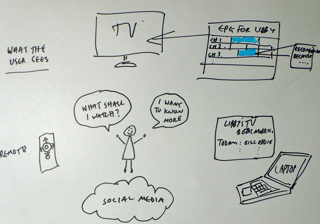
\includegraphics[width=6in]{review-demonstrator-description-1.png}
\caption{What the user sees} \label{fig:userview}
\end{center}
\end{figure}

\subsection{Physical Components}

The physical components are: 

\begin{itemize}
\item{Remote device (a smartphone)}
\item{TV set and media centre}
\end{itemize}


\begin{figure}[htbp]
\begin{center}
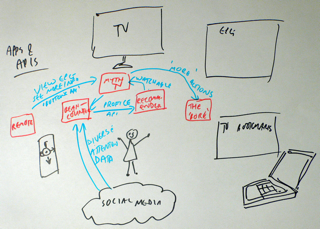
\includegraphics[width=6in]{review-demonstrator-description-2.png}
\caption{Applications and APIs} \label{fig:description}
\end{center}
\end{figure}

\subsection{Software Components}

The software components are: 

\begin{itemize}
\item{Remote control}
\item{MythTV or similar}
\item{Profiler (Beancounter)}
\item{Recommender (personalised content filter)}
\item{Various enhancement components, including enrichment and alignment services}
\end{itemize}

\section{Architecture}

\begin{figure}[htbp]
\begin{center}
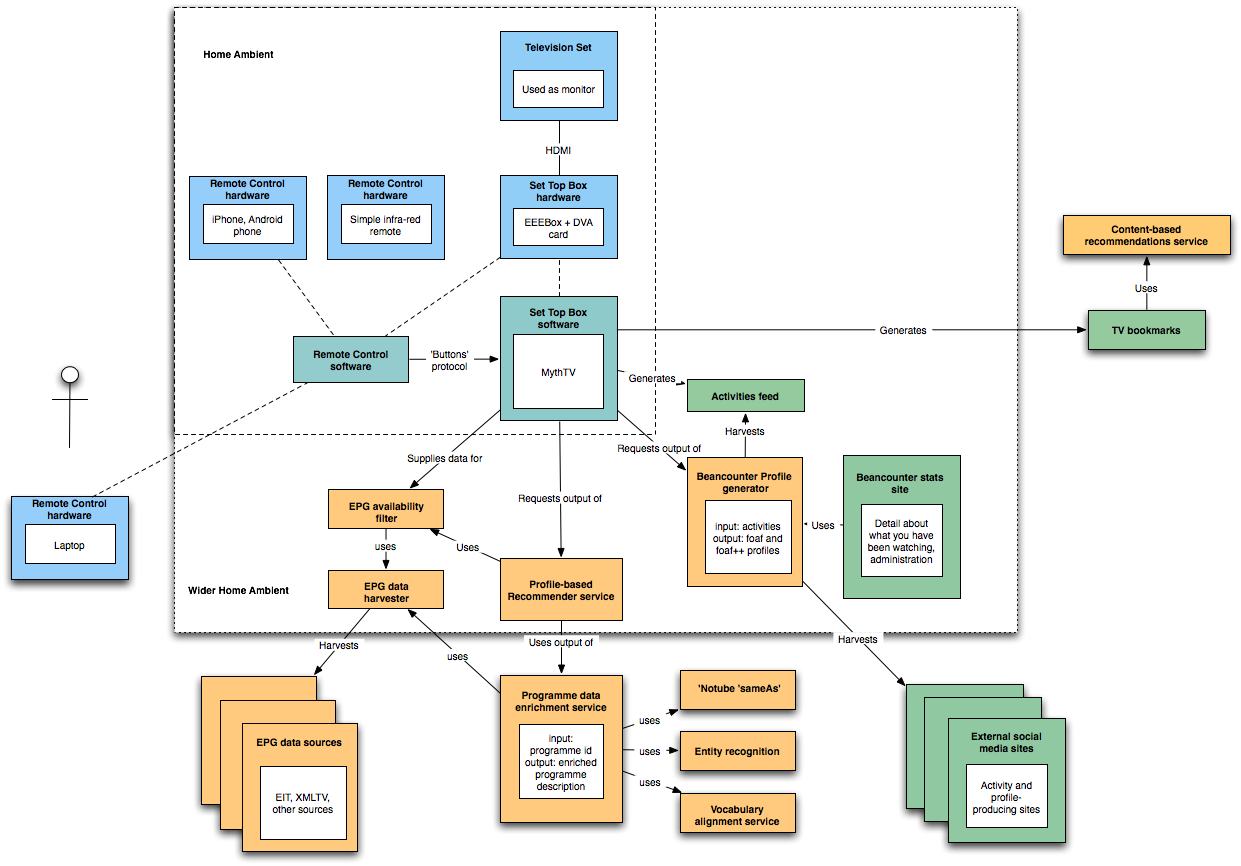
\includegraphics[width=7in]{architecture.png}
\caption{Architecture} \label{fig:architecture}
\end{center}
\end{figure}

The architecture is comprised of a set of services called by a sophisticated software media centre authorised by credentials sent from a smart phone acting as a remote control.

The user's remote `companion' device enables secure identification of the user to the media centre, which then can pass credentials from the device to other services such as the Beancounter and the recommender, which in turn use the various enhancement services.

It will be possible to run the beancounter and simple recommenders inside the home ambient for enhanced security and privacy, as the detailed architectural diagram Figure \ref{fig:architecture} shows.

\subsection{Scenario 1: Recommendations for me on my TV based on my web behaviour}

This scenario requires that the user pre-register on the Beancounter profiler, adding one or more sources of data from existing social media sites that she uses. When she comes home to her TV and media centre, she can view recommendations based on her Beancounter profile within the TV's programme guide (EPG), operating the media centre with her iPhone acting as a remote control. Profile access and recommendations for a given profile are via RESTful APIs, with security (if required) planned to be handled by OAuth.\footnote{\url{http://oauth.net/}}

Very important here for recommendations is the availability of programmes to the user. Broadcast content in particular is usually restricted to a particular geographical area, and some Web-based services like Hulu and iPlayer also restrict their content geographically. Similarly broadcast content is restricted by time (although there may be repeats) and some Web-based services also limit availability to a short period of time. A recommendations service must only recommend content available to the user.

Also important is the identification of channels and programmes to the user from the recommender to their media centre. Multiple formal and informal names for channels and programmes are used and a service to combine these is required (more in Scenario 3 below).

For the swimlane activity diagram, see Figure \ref{fig:swimlane1}, and for wireframes see Figure \ref{fig:wireframe1}, and see the Appendix for detailed scripts describing the process.

\begin{figure}[htbp]
\begin{center}
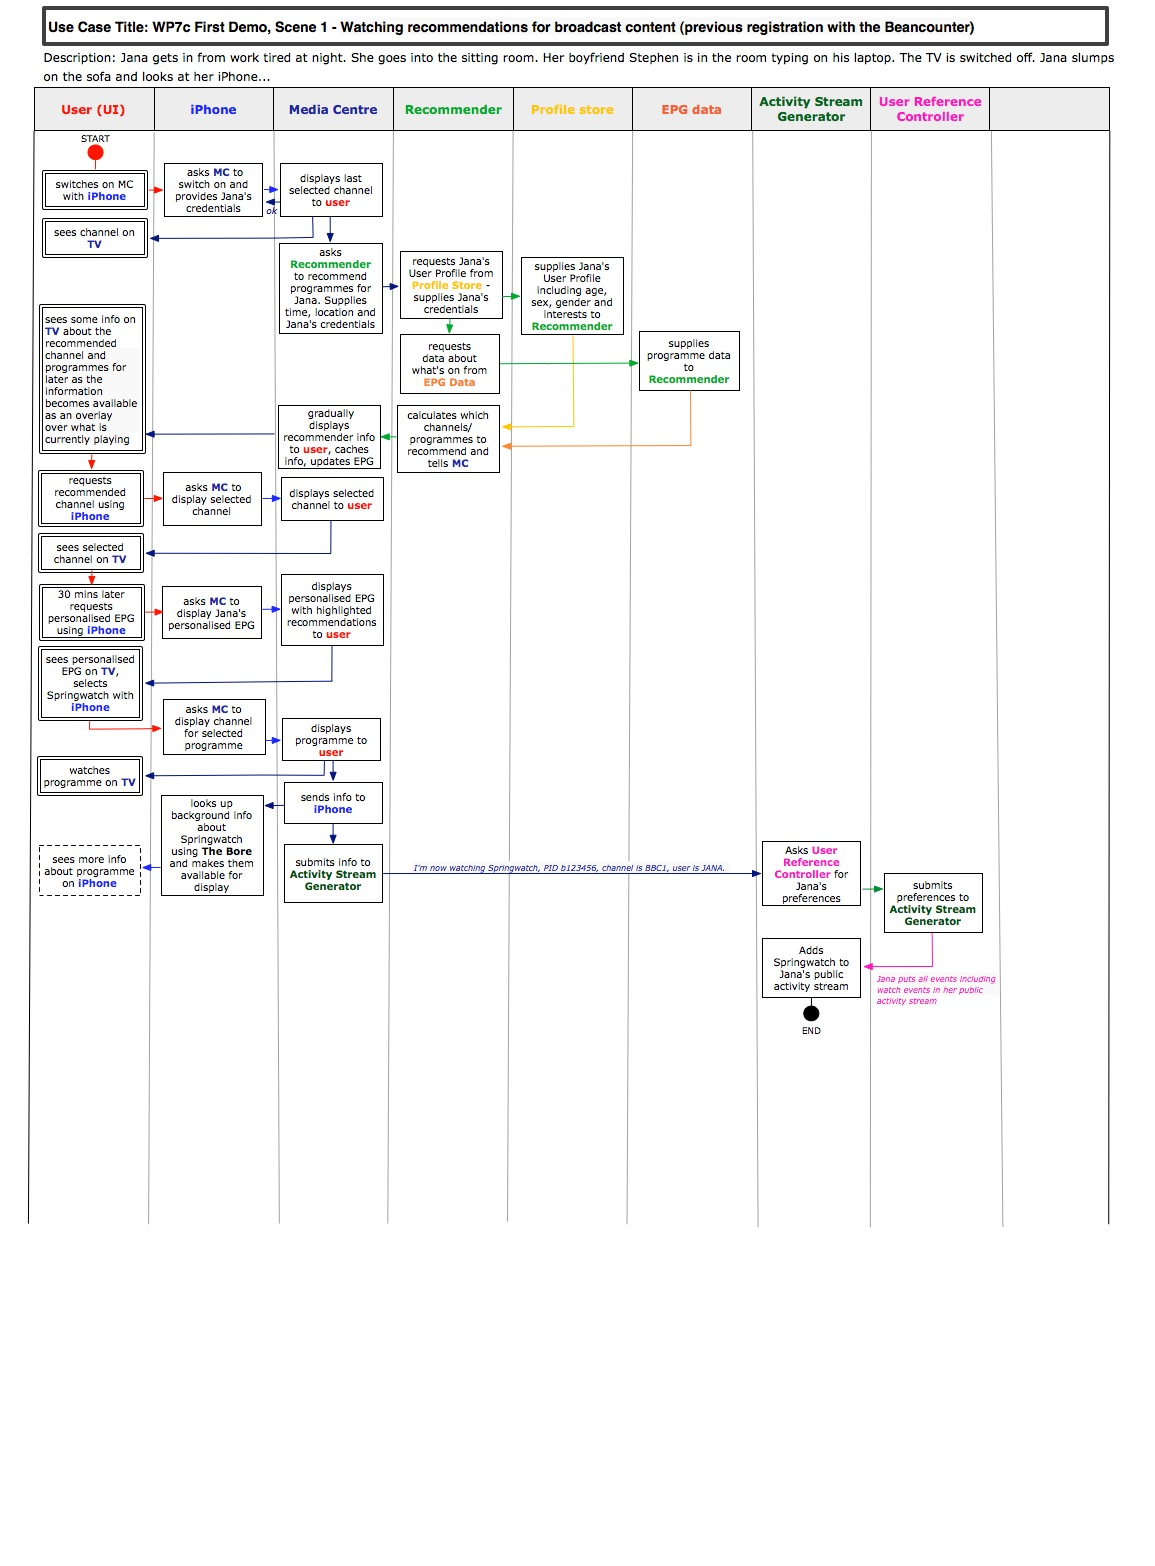
\includegraphics[width=6in]{WP7C_Demo_Swimlane_Script1.jpg}
\caption{Swimlane Scenario 1: The user chooses from recommendations on their TV screen using a smart phone acting as a remote control, connected to a media centre via XMPP. The user is able to view the EPG, change channel and view a programme.} \label{fig:swimlane1}
\end{center}
\end{figure}

\begin{figure}[htbp]
\begin{center}
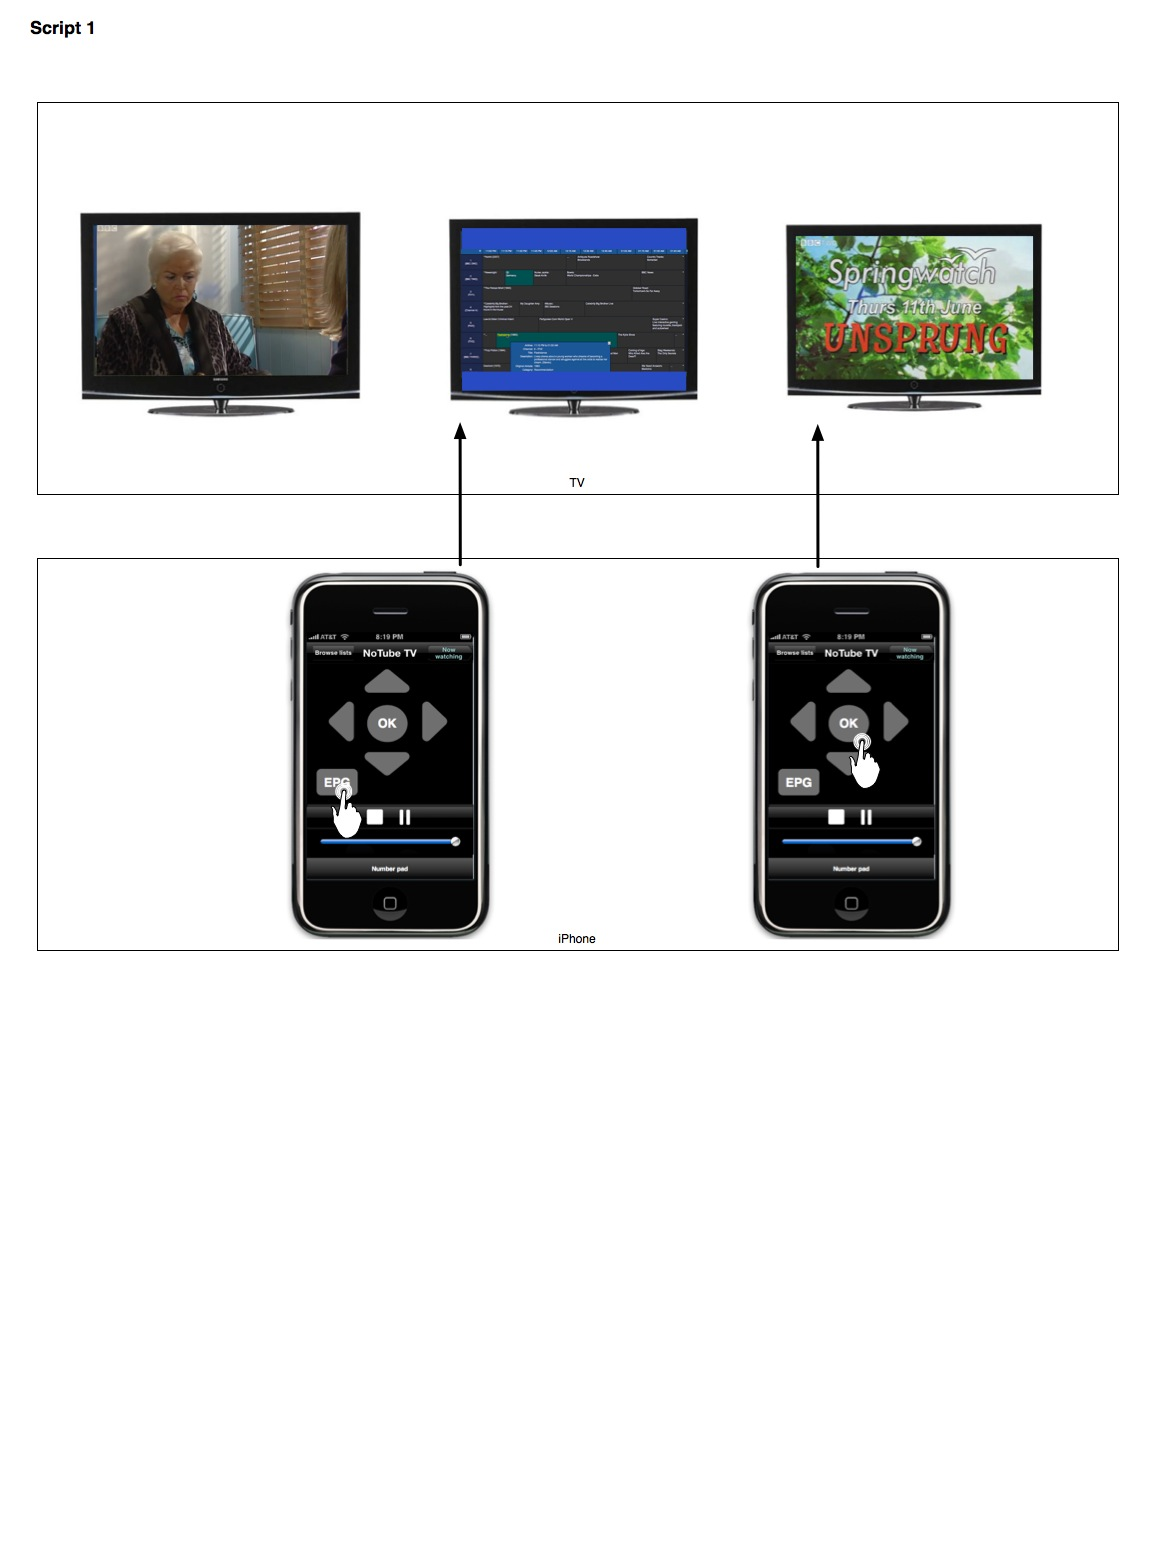
\includegraphics[width=5in]{Script_1_wireframes.jpg}
\caption{Wireframes Scenario 1: The user chooses from recommendations on their TV screen using a smart phone acting as a remote control, connected to a media centre via XMPP. The user is able to view the EPG, change channel and view a programme.} \label{fig:wireframe1}
\end{center}
\end{figure}


\subsection{Scenario 2: Do you want to know more?}

Scenario 2 is about finding more information automatically about a particular programme. Here we make use of the capabilities of the companion device to allow Jana to find out more information without disturbing anyone else in the room. An automated, linked-data service (which may include data enhancement services) can be employed to suggest interesting and novel information about a programme; if this is not available then basic data can be provided from a local or remote programmes data store.

Data enhancement services could include entity recognition for finding commonly used URLs for programmes, and `same as' functionality for linking various URLs about the same entity from across the linked data cloud. For example `Doctor Who' has the RDF (linked data) URL of \url{http://www.bbc.co.uk/programmes/b006q2x0.rdf}, in DBdedia it is \url{http://dbpedia.org/data/Doctor_Who.rdf}, in Freebase \footnote{\url{http://www.freebase.com/}} it is \url{http://rdf.freebase.com/rdf/en.doctor_who} and in IMDB (not part of the linked data cloud but commonly used to refer to Film and TV entities) it is \url{http://www.imdb.com/title/tt0436992/}. 

An additional part of the problem is very similar to the linked data recommendations issue referred to above: finding {\bf interesting} items through a cloud of links requires some filtering; this is important an area of research for the project.

Architecturally, we have chosen to link the media centre with the remote using the XMPP `buttons' protocol\footnote{\url{http://wiki.foaf-project.org/w/Buttons}}, where the media centre has its own XMPP-addressible unique identifier which has the notion of trusted contacts. This potentially solves some of the security and privacy issues raised in scenario 3 and in more detail below. 

For swimlane activity diagram, see Figure \ref{fig:swimlane2}, and for wireframes see Figure \ref{fig:wireframe2}, and again, see the Appendix for detailed scripts describing the process.

\begin{figure}[htbp]
\begin{center}
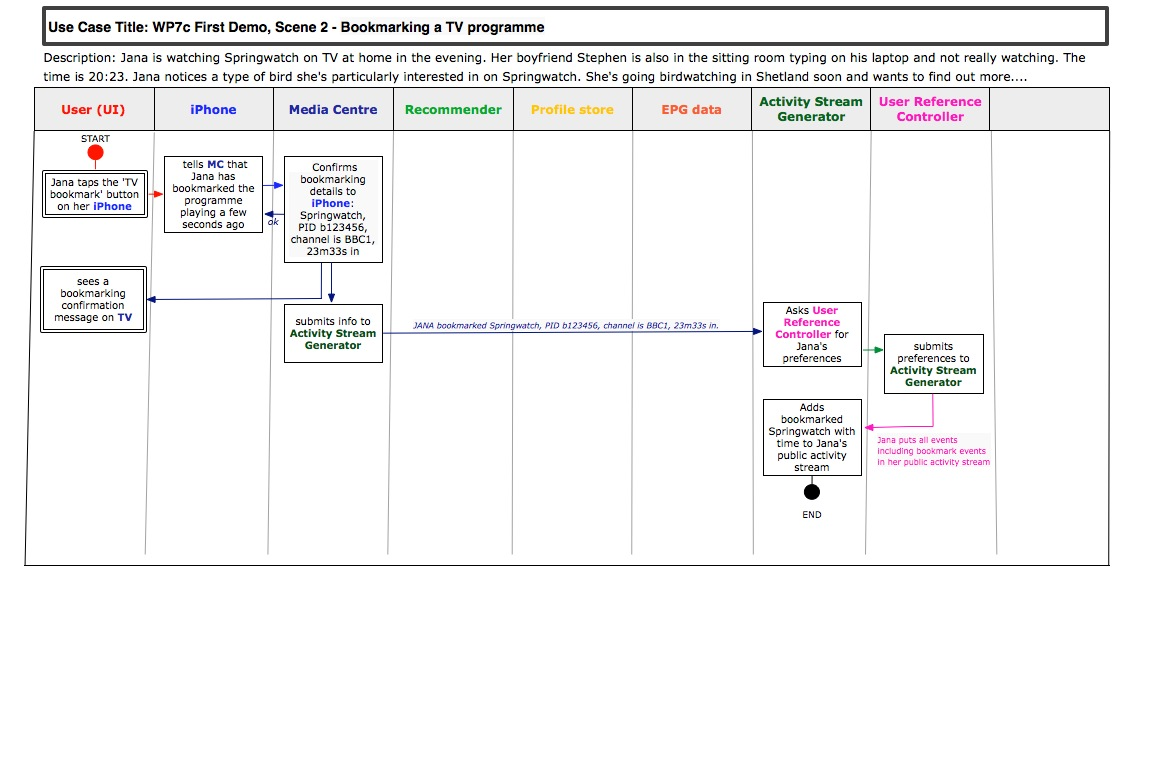
\includegraphics[width=6in]{WP7C_Demo_Swimlane_Script2.jpg}
\caption{Swimlane Scenario 2: The user uses the smart phone remote to bookmark a programme which is then sent out to the Web} \label{fig:swimlane2}
\end{center}
\end{figure}

\begin{figure}[htbp]
\begin{center}
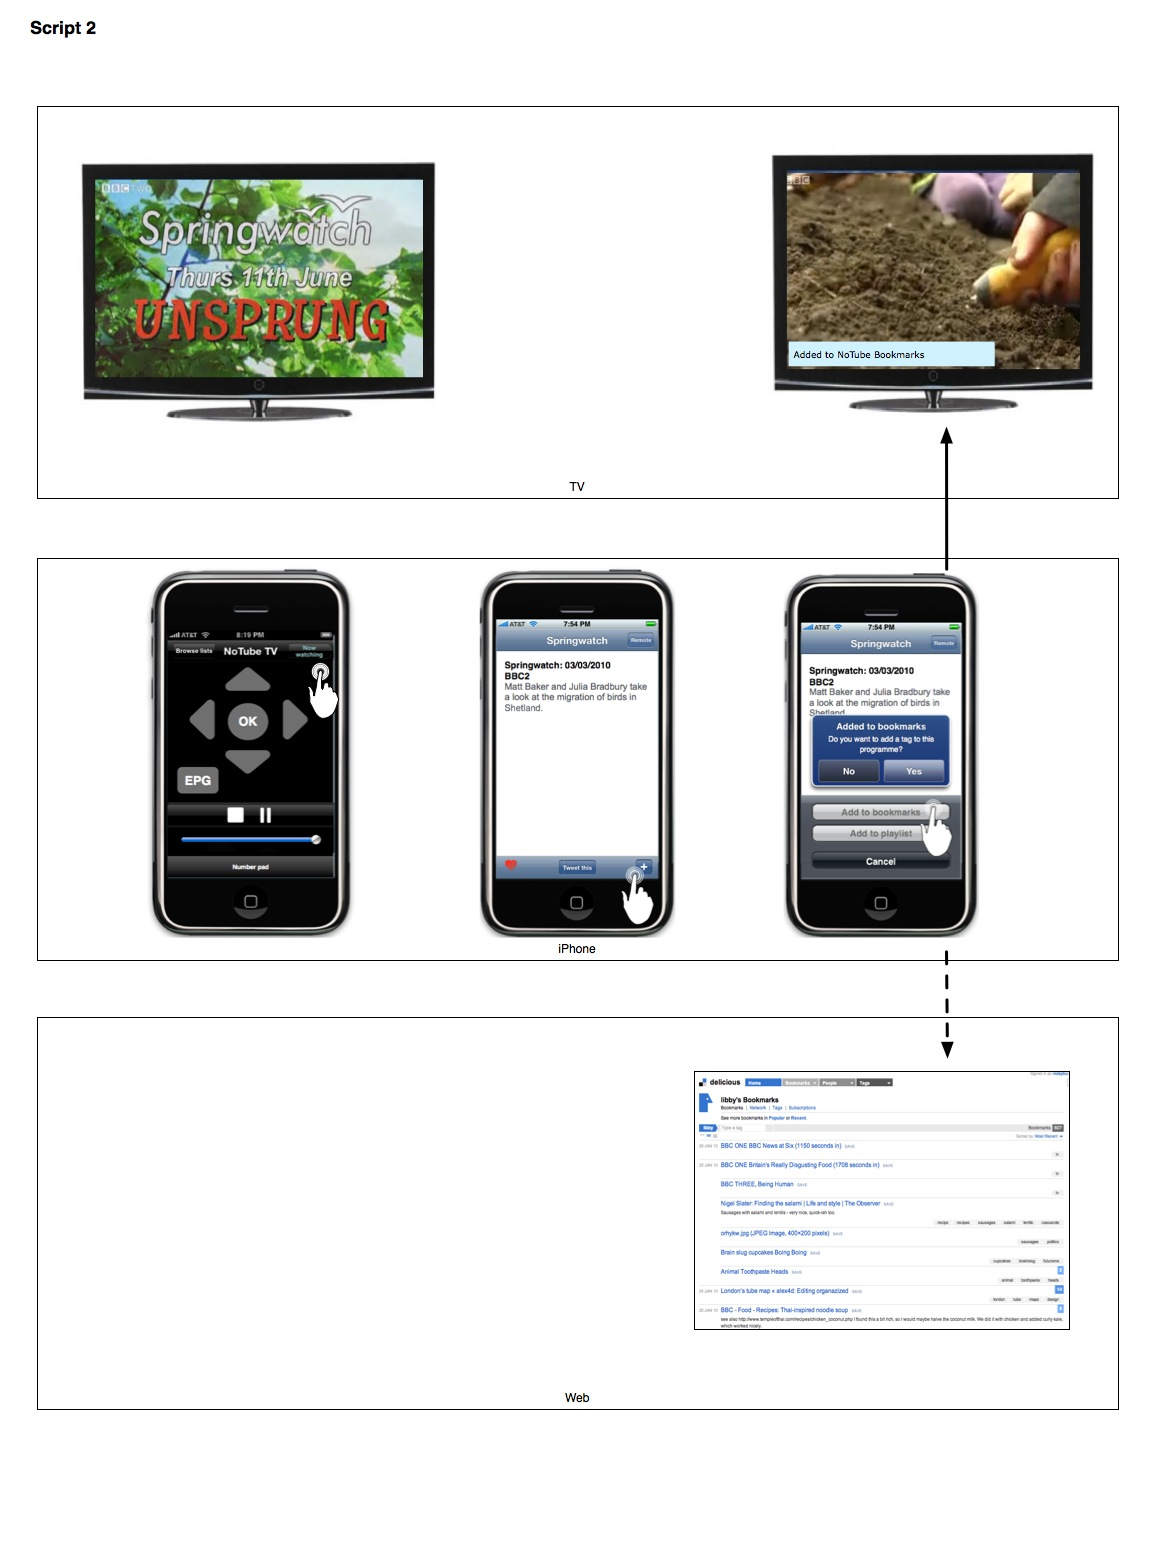
\includegraphics[width=5in]{Script_2_wireframes.jpg}
\caption{Wireframes Scenario 2: The user uses the smart phone remote to bookmark a programme which is then sent out to the Web} \label{fig:wireframe2}
\end{center}
\end{figure}


\subsection{Scenario 3: Add to media centre's `to watch' list, while away from Local Area Network}

In Scenario 3, the user receives news of interesting media in of a context when he cannot easily watch it. The most obvious example is via social media, where the user's friends may tell him about programmes of interest that he cannot or does not want to consume immediately but might be interested to watch when he is more comfortable at home. These social networking news items are often transient and so remembering for later is useful. They commonly use Web URLs as a means to describe programmes, although sometimes shorthand names for TV channels or just the titles of programmes may be used. This scenario is particularly relevant to long-form content rather than short pieces of video.

This functionality requires well-defined APIs connecting the media centre within the `home ambient' and the wider network, together with appropriate authentication and security mechanisms to prevent unauthorised high-resource-consumption downloads. 

It also requires well-defined descriptors for programmes and channels which are usable and accessible on the Web {\bf and} from a media centre. In some cases a URL is sufficient for both of these but in other cases there need to be mappings made between formal names (e.g. DVB 'CRIDs' or BBC programmes or iPlayer URIs), informal names (often as `tags') and persistent or transitory URLs for programmes and channels. There may also be a need for services that can be used to determine what was on at a particular time on a particular channel, title resolvers and other data enhancement services that enable reference to the same item of interest.

For the swimlane activity diagram, see Figure \ref{fig:swimlane3}, and for wireframes see Figure \ref{fig:wireframe3}.

\begin{figure}[htbp]
\begin{center}
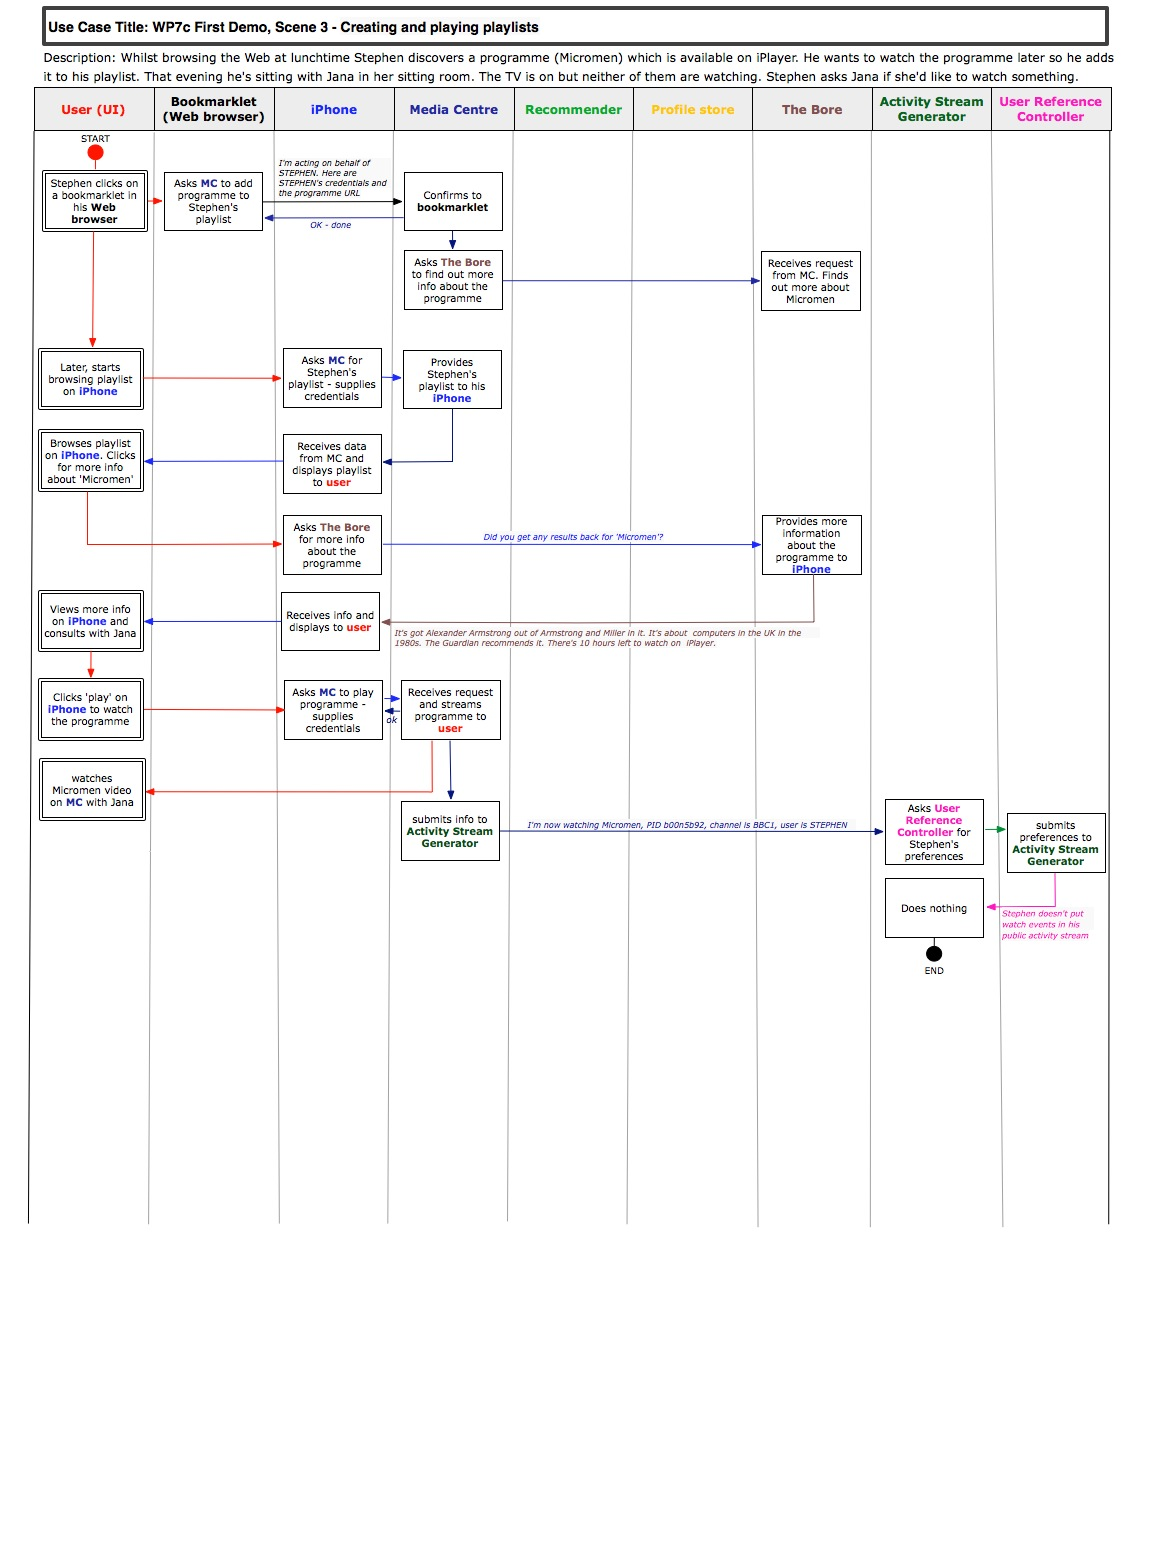
\includegraphics[width=6in]{WP7C_Demo_Swimlane_Script3.jpg}
\caption{Swimlane Scenario 3: The user adds a programme to his `to watch' list while at work, and then uses the smart phone remote to navigate to it  and play it when at home.} \label{fig:swimlane3}
\end{center}
\end{figure}


\begin{figure}[htbp]
\begin{center}
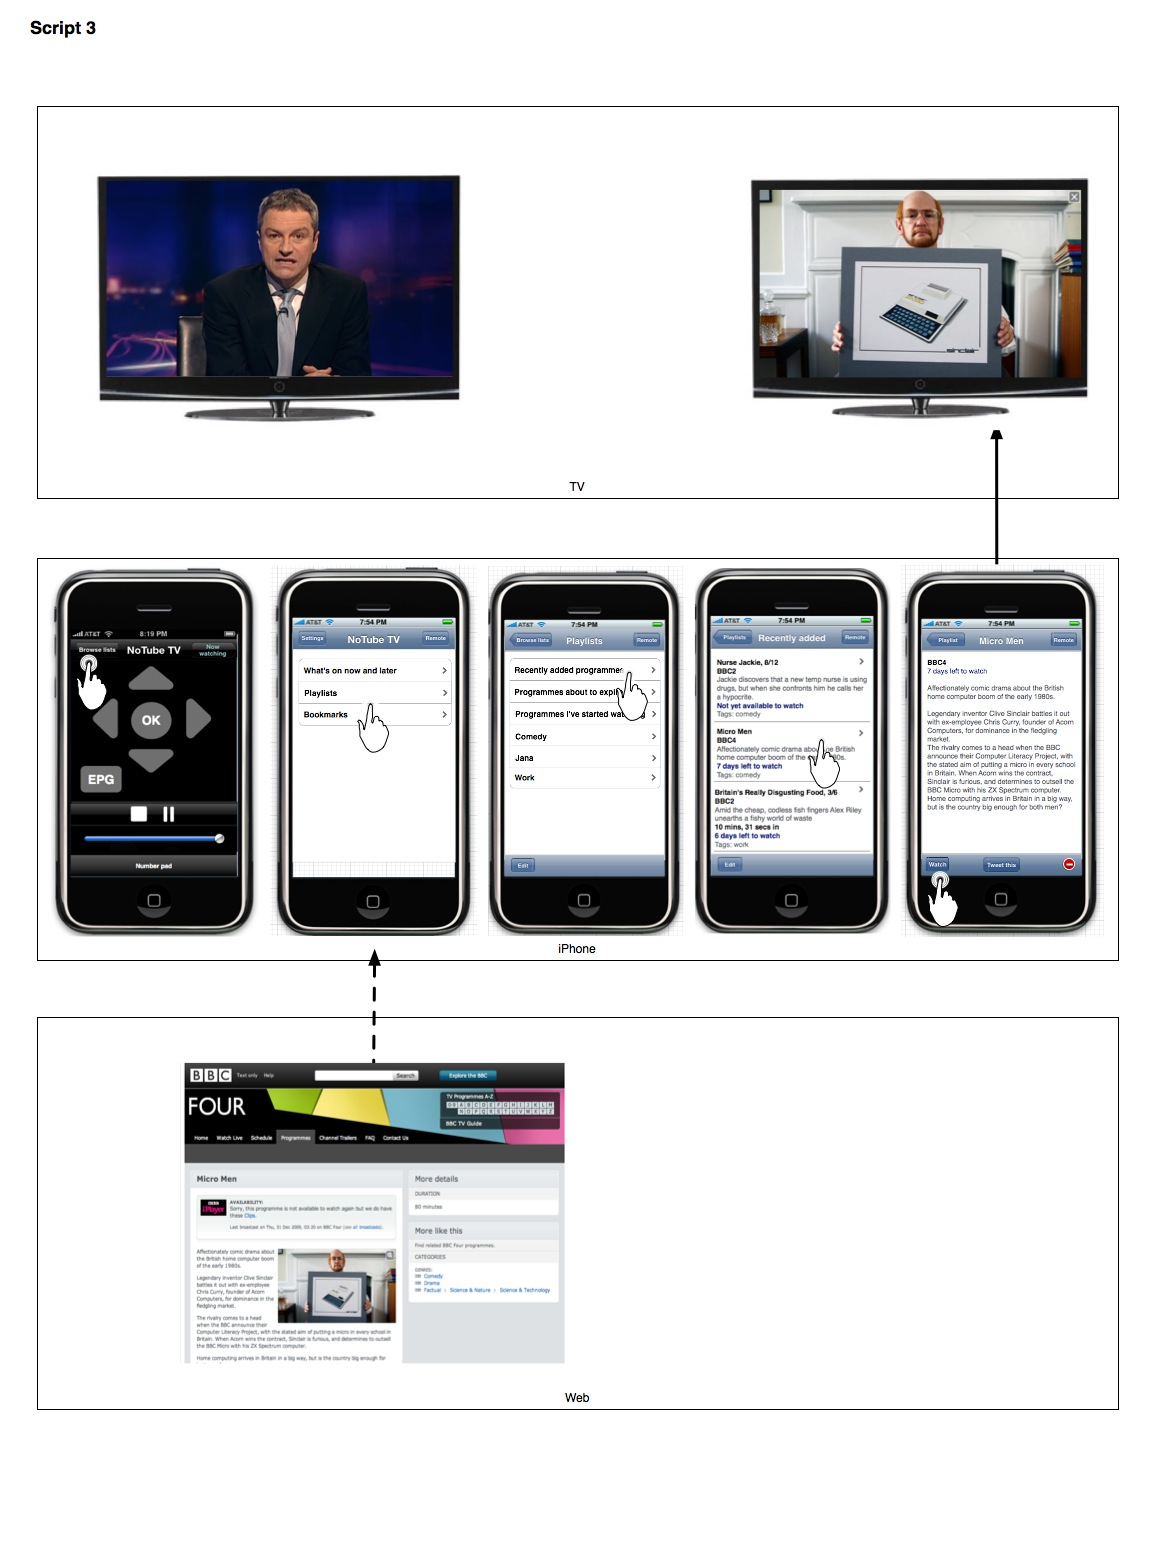
\includegraphics[width=5in]{Script_3_wireframes.jpg}
\caption{Wireframes Scenario 3: The user adds a programme to his `to watch' list while at work, and then uses the smart phone remote to navigate to it  and play it when at home.} \label{fig:wireframe3}
\end{center}
\end{figure}


\chapter{Requirements}

These come under the following headings:

\begin{itemize}
\item{User Experience}
\item{Security and Privacy}
\item{Devices}
\item{Software components}
\begin{itemize}
\item{Profiler (Beancounter)}
\item{Recommender (personalised content filter)}
\item{Data Enhancement}
\end{itemize}
\end{itemize}

\section{User Experience}

The main principles are that:
\\

\begin{center}
 \begin{tabular*}{1.00\textwidth}{ | p{1.6cm} | p{4cm}| p{8.5cm} | }
    \hline
    R1.1 & The user is identified by their device & To minimise authentication input from the user by using the device to identify them. \\ \hline
    R1.2 & Changes to media centre UI should be minimal & It is not practical or sensible to create our own media centre. All efforts should be on open source projects and should be contributed back to the project if possible. Services and devices should be found automatically by the box. Recommendations should be a question of reordering (on demand) or highlighting (EPG)\\ \hline
    R1.3 & Major device events should be visible onscreen (as an unobtrusive `bug') & To give the user feedback, for example when a new device assumes control or a bookmark is created.\\ \hline
    R1.4 & Devices once enabled can have lots of control & To draw on the advantages of input using devices designed for textual input, such as computers and to a certain extent phones, versus devices that are very poor at handling textual input such as televisions and media centres. \\ 
    \hline
\end{tabular*}
  \captionof{table}{User Experience Requirements}
  \label{table1}
\end{center}


\section{Security and Privacy Requirements}

Security and privacy are important parts of a system which uses multiple services and deals with personal data, particularly in a shared environment such as a TV. Many of the privacy considerations arise from the use of the Beancounter profiler and these are detailed in D3.1. However there are specific security and privacy requirements coming directly from the interaction of the device and media centre. 
\\
\begin{center}
\begin{tabular*}{1.00\textwidth}{ | p{1.6cm} | p{4cm}| p{8.5cm} | }
    \hline
    R2.1 & The device must be able to detect suitable media centres and alert the user in a non-intrusive fashion & Ideally it should detect them automatically.\\ \hline
    R2.2 & The device should be able to detect the capabilities of the media centre & For example, can it pause / play? are there privacy settings? can it stream video?\\ \hline
    R2.3 & The device must be able to securely `pair' with the media centre & For example: Jana enters the room; her device detects the media centre, and some interaction takes place so that both devices know that they are genuinely talking to each other and can continue to trust one another subsequently. As a first pass, we can simply trust all devices on the Local Area Network or else pre-coordinate the trust relationships.\\ \hline
    R2.4 &The device must be able to identify itself to the media centre & It needs a unique identifier that is persistent over sessions.\\ \hline
    R2.5 & The device must be able to send identity credentials for other applications securely & For example: Jana's phone has enough credentials to allow the media centre to be able to identify her to the recommender application. The media centre takes the credentials that Jana sends with her phone and passes them securely to other applications. This could of course be achieved by Jana sending her username and password via the media centre to the recommender, but that's far from ideal. What we want is something that the phone gives the media centre that allows the media centre to identify as Jana\\ \hline
   R2.6. & The Media Centre must be able to securely pass credentials to other services & (see above)\\ \hline
   R2.7 & The Media Centre must allow non-LAN connections to securely update its playlist & For example the user could be at work when they find interesting items to look at later.\\
    \hline
  \end{tabular*}
  \captionof{table}{Security and Privacy Requirements}
  \label{table2}
\end{center}

\section{Media Centre Requirements}

The aims are:

\begin{itemize}
\item{A box that can perform the usual TV functions, including broadcast TV}
\item{Can be modified, for example to use a separate device as a remote or to add new metadata creation functionalities}
\end{itemize}

The Media Centre must be able to do the following:
\\
\begin{center}
\begin{tabular*}{1.00\textwidth}{ | p{1.6cm} | p{4cm}| p{8.5cm} | }
    \hline
R3.1 & Play live TV & For example via DVB-T\\ \hline
R3.2 & Play on demand TV & For example from a local file.\\ \hline
R3.3 & Display programme guide (EPG) & Show what's on live TV now and in the future ideally in a grid-based (time-based) format.\\ \hline
R3.4 & API to video use and navigation parameters & For example XBMC has an http API; MythTV frontend has a sockets based API.\\ \hline
R3.5 & Have the ability to modify appearance of displays & In particular the programme guide (EPG) to show recommendations, and the on demand playlist to show recommendations and to add items using an API.\\ \hline
R3.6 & Should have the ability to display text onscreen & In order to subtly alert the user when an important action has taken place using the remote.\\ \hline
R3.7 & Have the ability to notify devices of events & For example, when a user starts watching a programme, the device is notified what she is watching.\\ \hline
R3.8 & Have the ability to make changes and additions to the code & To add prototype additions:\\ \hline
R3.8.1 & Minor UI changes & Highlighting and on screen messages.\\ \hline
R3.8.2 & Activities streams additions & Including privacy settings, activities streams output.\\ \hline
R3.8.3 & XMPP protocol additions & Implementation of the Buttons protocol for remote functions and security related functions.\\ \hline
R3.8.4 & HTTP additions & For example to display activity streams, query the local EPG for data about upcoming showings of recommended programmes.\\ \hline
R3.9 & An API to these functionalities & We may need to create some of these API calls ourselves.\\ \hline
R3.10 & Secure LAN and non-LAN network access & For updating and querying the system remotely.\\
    \hline
  \end{tabular*}
  \captionof{table}{Media Centre Requirements}
  \label{table3}
\end{center}


\section{Remote device requirements}

The aims are:
\\
\begin{itemize}
\item{A user experience that will work for both iphone and web-on-iphone or web-on-other-small-device}
\item{A remote that does four groups of things: }
\begin{itemize}
\item{Basic remote functions for playing and navigating broadcast and ondemand TV}
\item{View and use configuration and privacy preferences for the media centre}
\item{View and use information about what is on now and later}
\item{View and use information about what is being watched now}
\end{itemize}
\end{itemize}

\begin{center}
\begin{tabular*}{1.00\textwidth}{ | p{1.6cm} | p{4cm}| p{8.5cm} | }
    \hline
R4.1 & Basic remote & Here the UI on the remote is basic and causes UI events on the screen. \\ \hline
R4.1.1 & Navigate up / down / left / right and select (`ok') & For selecting items on the media centre screen within the programme guide (EPG) or navigating other lists.\\ \hline
R4.1.2 & On-screen EPG navigation &  \\ \hline
R4.1.3 & On-screen Tree-based navigation &  \\ \hline
R4.1.4 & basic video controls (play, pause, rewind, fast forward) & To control the video on the media centre screen.\\ \hline
R4.1.5 & Information & Show information about the item being watched.\\ 
    \hline
  \end{tabular*}
  \captionof{table}{Basic Remote Requirements}
  \label{table4}
\end{center}
\begin{center}
\begin{tabular*}{1.00\textwidth}{ | p{1.6cm} | p{4cm}| p{8.5cm} | }
    \hline
R4.2 & Bookmark & This should allow the user to enter some information about the bookmark (such as tags) on the remote itself, and this action may optionally have a small effect on the TV (such as a little `bug' in the corner saying `bookmark created'). \\ \hline
R4.3 & Add to Playlist & There are two situations in which the user may want to add to her playlist (our list of on-demand items) using the remote\\ \hline
R4.3.1 & Add to playlist from a programme being viewed & She sees an advert for something on the TV. This is a future usecase, but an important one\\ \hline
R4.3.2 & Add to Playlist from a Webpage & This should be treated the same as the case where we are at our desk browsing the web and see something interesting, i.e. some sort of additional button on the webpage and some sort of response (such as a javascript popup or similar) to say that it has been added to the playlist.\\ 
    \hline
  \end{tabular*}
  \captionof{table}{New Remote Requirements}
  \label{table5}
\end{center}

\begin{center}
\begin{tabular*}{1.00\textwidth}{ | p{1.6cm} | p{4cm}| p{8.5cm} | }
    \hline
R4.4 & Media Centre privacy preferences and configuration options & If the device has a high level of trust, it can access the internal configuration of the media centre for that user, in particular privacy and notification settings, taking advantage of being able to input text more effectively on the device than on the TV. The main parts are:\\ \hline
R4.4.1 & Make all events (user activity logs and notifications) private & \\ \hline
R4.4.2 & Make all events public &  \\ \hline
R4.4.3 & Make all events except `watch' public &  \\ \hline
R4.4.4 & Delete all events & There are some significant issues here around `delete' and whether it would apply to all the events coming from the box or just ones associated with my control over the box? There are also currently unknowns around how we allow the device to be trusted (see below).\\ \hline
R4.5 & Notification settings & \\ \hline
R4.5.1 & Enable notifications to device & \\ \hline
R4.5.2 & Disable notifications to device & Notifications in this sense are when channel changes happen or bookmarks happen the device may want to update itself (see below).\\ \hline
R4.6 & Connection settings &  \\ \hline
R4.6.1 & Detect services &  \\ \hline
R4.6.2 & Create a connection with media centre &  \\ \hline
R4.6.3 & Show connections & \\
    \hline
  \end{tabular*}
  \captionof{table}{Settings Remote Requirements}
  \label{table6}
\end{center}


\section{EPG on Remote Requirements}

The idea here is that the user may look at the EPG on their device rather than the media centre, and look for things to watch immediately without disturbing others. There are many apps that allow you to browse EPGs like this, though none we know of that allow you to also change channel. Later we may want to add the ability to create reminders for broadcast data using this functionality.

\begin{center}
\begin{tabular*}{1.00\textwidth}{ | p{1.6cm} | p{4cm}| p{8.5cm} | }
    \hline
R5.1 & View EPG & What's on now and later \\ \hline
R5.2 & Scroll & To see programmes that are on later \\ \hline
R5.3 & View information & About a show \\ \hline
R5.4 & Change channel & To a show \\
    \hline
  \end{tabular*}
  \captionof{table}{EPG on Remote Requirements}
  \label{table7}
\end{center}


\section{Detailed Information on Remote Requirements}

The idea is that if notifications are switched on, the device knows what is playing on the media centre and can update itself accordingly with information about the show, for example from the linked data web. It is important that however this information is displayed, it is not too difficult to navigate from this to other webpages so that the user can talk to others about what she is watching, find out more information, follow links etc.

\begin{center}
\begin{tabular*}{1.00\textwidth}{ | p{1.6cm} | p{4cm}| p{8.5cm} | }
    \hline
R6.1 & See information about what is playing on the media centre & View this information on the remote device. \\ \hline
R6.2 & Navigate away from it & I.e to webpages. \\
    \hline
  \end{tabular*}
  \captionof{table}{Detailed Information on Remote Requirements}
  \label{table8}
\end{center}

\section{Profiler Requirements}

The profiler (`Beancounter') allows the user to generate a machine-processible summary profile of their interests, preferences and dislikes using data aggregated from various social media sources that they already use. It is used as input to a recommender (see below) that can suggest programmes to the user, for example in the first scenario by displaying an EPG with highlighted recommendations. Much more detail about the Beancounter profiler is available in D3.1.
\\

General considerations:

\begin{center}
\begin{tabular*}{1.00\textwidth}{ | p{1.6cm} | p{13cm} | }
    \hline
R7.1 & Must allow users to create accounts \\ \hline
R7.2 & Must allow users to add and remove social data accounts to their beancounter account \\ \hline
R7.3 & Must output an RDF profile (in the format described in the Appendix below) \\ \hline
R7.4 & Must provide access to the raw activities data \\ \hline
R7.5 & Must provide access to the aggregated activities data \\ \hline
R7.6 & Must provide secure access to any private data\\ 
    \hline
  \end{tabular*}
  \captionof{table}{Profiler General Requirements}
  \label{table9}
\end{center}

User Interface and privacy considerations:

\begin{center}
\begin{tabular*}{1.00\textwidth}{ | p{1.6cm} | p{4cm}| p{8.5cm} | }
    \hline
R7.7 & By default all Profile data should be private until the user actively chooses to share it & \\ \hline
R7.8 & The user can only `share' their Beancounter Profile from the screen where they can see their Profile & This is to protect the user from sharing things which they may prefer to keep private.\\ \hline
R7.9 & Any updates or changes to the Profile are private by default & The user can be alerted to changes by email if they choose to subscribe. If not, there is an �updated� icon on the Profile screen and facility to see most recent changes. The user must approve any updates before they are shared.\\ \hline
R7.10 & Users must be able to edit their Profiles at any time & (e.g. to delete / hide / strengthen / weaken specific topics) \\ 
    \hline
  \end{tabular*}
  \captionof{table}{Profiler UI Requirements}
  \label{table10}
\end{center}

\section{Personalised Filter (Recommender) Requirements}

The recommender or personalised filter is some means to turn a list of of a user's interests, preferences and dislikes into a list of available on-demand or broadcast programmes to watch. 

\begin{center}
\begin{tabular*}{1.00\textwidth}{ | p{1.6cm} | p{13cm} | }
    \hline
R8.1 & Must take as input a profile(see Appendix below)\\ \hline
R8.2 & Must be able to connect to a profile generator securely with a username and password or oath token, OR be able to connect to a profile generator with a username for public data|\\ \hline
R8.4 & Must allow retrieval of data using username and password, or just username for public data\\ \hline
R8.5 & Must output a list of URIs with channels, dates of broadcast or availability and rationales (explanation of why something was recommended) (see Appendix below)\\
    \hline
  \end{tabular*}
  \captionof{table}{Personalised Filter (Recommender) Requirements}
  \label{table11}
\end{center}


\section{Data Enhancement Requirements}

As part of its website the BBC aims to produce a URL for each programme created, available in HTML and RDF formats, and linked to other items of interest, such as series, genre and contributors, using the BBC Programmes Ontology\footnote{\url{http://www.bbc.co.uk/ontologies/programmes/}} and in some cases MusicBrainz and DBpedia identifiers. In doing so it forms part of the Linked Data Cloud. This is separate to its iPlayer catchup service, although where video of the programme is available it will be linked from or embedded in the programme page.

This makes for a useful testbed for these ideas: without adding to the BBC data, we can easily create bookmarking systems, because there has a URL for most recent programmes - for the BBC, TV already links to the Web. In addition, because the BBC Programmes Ontology is an FRBR-based vocabulary, it distinguishes between items of interest at the `Brand' (e.g. Doctor Who), `Series' (e.g. Doctor Who Series 8), `Programme' (Doctor Who Series 8, episode 5'), `Version'  (Doctor Who Series 8, episode 5 with signing). It also describes when it was broadcast, the genre it is placed in. and in some cases who the contributors were. This means that extremely simple recommendations such as 'you might like this episode of Doctor Who because you liked the series Doctorr Who Series 8' can be made using this data alone, using the identifiers and the broadcast schedule.

For more interesting and for non-BBC content suggestion and filtering there is substantial work to be done in 

\begin{center}
\begin{tabular*}{1.00\textwidth}{ | p{1.6cm} | p{13cm} | }
    \hline
R9.1 &Concept identification: creating new links between items of interest and other vocabularies, using natural language processing or ontology matching\\ \hline
R9.2 &Matching different identifiers for the same item. In the example of the database on the Web, where there are different unique keys coming form different databases which refer to the same thing, we need to find them and create links between them. An example might be a BBC programme URL for Murder She wrote, Series 12, episode 4 and the equivalent IMDB URL.\\ \hline
R9.3 &Matching of schedule and TVAnytime broadcast identifiers and Web programme identifiers\\ \hline
R9.4 &Matching user channel or programme availability to any given user, for example using schedule data and location data\\ \hline
R9.5 &Generated or existing URLs for channels and programmes\\ 
    \hline
  \end{tabular*}
  \captionof{table}{Data Enhancement Requirements}
  \label{table11}
\end{center}


\chapter{Prototype}

\section{User Experience}

User experience is a key component of the prototype. We have created diagrams (see below) illustrating the structure of the interactions the user has with the various devices. The initial remote device we will implement for is an iPhone or iPod touch (both provide more or less the same functionality). The functions are designed to be be implemented using an application or a webpage, and we may do both. 

The most important aim here is to help the user distinguish between cases where the remote is acting as a remote (for example when Jana uses it to change channels or navigate an EPG on the media centre screen) and cases where it is acting as a companion device (for example to see more information about a programme, or to browse an EPG privately). This could be extremely confusing for the user, and we do not know whether this will make the idea unusable.

\subsection{Functioning as a remote}


\begin{center}
\begin{tabular*}{1.00\textwidth}{ | p{1.6cm} | p{13cm} | }
    \hline
R9.1 & TV remote functions (show EPG, left, right, up, down, select, play, stop, vol up/down) must be clearly separated from other functions (i.e. those not related to changing what's happening on the TV screen). This will probably be via use of consistent navigation buttons in the pane. \\ \hline
R9.2 & The TV remote functions part of the design should be as simple as possible. It should also be inspired by existing similar remotes so as to be familiar. \\ 
    \hline
  \end{tabular*}
  \captionof{table}{Remote Interface User Experience (UX) Requirements: Functioning as a remote}
  \label{table12}
\end{center}


\subsection{Functioning as a companion device}


\begin{center}
\begin{tabular*}{1.00\textwidth}{ | p{1.6cm} | p{4cm}| p{8.5cm} | }
    \hline
R9.3 & The device must be able to display a programme guide (EPG) showing what's on now and later & This is a local version of the personalised EPG displayed on the remote (this is the same info as displayed on the Media Centre although presented differently) for scenarios where the user does not want to interrupt what's showing on the TV screen because there are other people watching the TV.  \\ \hline
R9.4 & The device must be able to display multiple lists of programmes (playlists) & These are programmes of interest that the user has either added via a Web browser bookmarklet (e.g. from an IPlayer page or a /programmes page as described in Script 3) or has indicated that they want to watch later (via the EPG) or was half-way through watching and wants to finish watching at some later point in time. The playlists are about finding previously flagged on-demand (or recorded) content to watch if there's nothing interesting on TV. Programmes can be tagged to create the playlists.  \\ \hline
R9.5 & The device must be able to differentiate between these playlists and the items the user has expressed an interest in finding out more background information about & This `find out more list' is about reading more information about a programme - either after watching a programme of interest (the `arctic tern' example in Script 2) or when deciding whether to start watching a a programme (the `Micromen' example in Script 3). This differentiates it conceptually from the Playlists (which are about watching things). \\
    \hline
  \end{tabular*}
  \captionof{table}{Remote Interface User Experience (UX) Requirements: Functioning as a companion device}
  \label{table13}
\end{center}


\subsection{Navigating and using lists}


\begin{center}
\begin{tabular*}{1.00\textwidth}{ | p{1.6cm} | p{13cm} | }
    \hline
R9.6 & Programmes in playlists that the user is half-way through watching must be distinguished visually from other lists of programmes \\ \hline
R9.7 & These must clearly show the timestamp (e.g. 10 mins 33 secs in) in the display.  \\ \hline
R9.8 & When a programme of this type is selected a dialogue box will allow the user to start watching the programme again from the beginning or to continue watching it from where they left off.  \\ \hline
R9.9 & Programmes of this type should be automatically tagged `programmes I'm half-way through' (or similar) for easy identification in the playlists. \\ \hline
R9.10 & Programmes in all playlists will clearly display expiry info - e.g. `7 days left to watch' where available.  \\ \hline
R9.11 & The user should be able to sort programmes in playlists by `most recently added' and `least time left to watch'  \\ \hline
R9.12 & Tapping on a list item should move the screen to the left if an iphone application. \\ \hline
R9.13 & Tapping on a list item must display more details for example from /programmes data  \\ \hline
R9.14 & Action buttons - e.g. watch, add to playlists, read more should be in a fixed position on screen \\
    \hline
  \end{tabular*}
  \captionof{table}{Remote Interface User Experience (UX) Requirements: Navigating and using lists}
  \label{table14}
\end{center}


\chapter{Current Status and Future Work}

\section{Current Status}

Currently we have proof-of-concept demonstrations illustrating the first two scenarios, plus the accompanying detailed documentation of the scenarios including the swimlanes and wireframes, which put us in a  good development position.

\subsection{Scenario 1: View Recommendations in an EPG}

The screenshots in Figures \ref{fig:mythtv-recommendations} and \ref{fig:mythweb-recommendations} show recommendations appearing as a changed UI in MythTV frontend media centre and its web-based navigator. This shows that the UI can be altered, and in building it we discovered the fields we needed for the output of the recommendations engine: a consistent channel identifier and an exact date-time value.

We also ran into issues of selection of content for recommendation, requiring a service that enables a list of programmes (`The Simpsons episode number 5427', `Doctor Who Series 8, episode 5') to be transformed into a brands (for example `The Simpsons', `Doctor Who') and then again into upcoming instances of programmes. We therefore require time and schedule information localised to the viewer so that they can actually watch it. That is, even if you know what you are recommending for someone, you still need to be able to tell them if and when it is available.

\begin{figure}[htbp]
\begin{center}
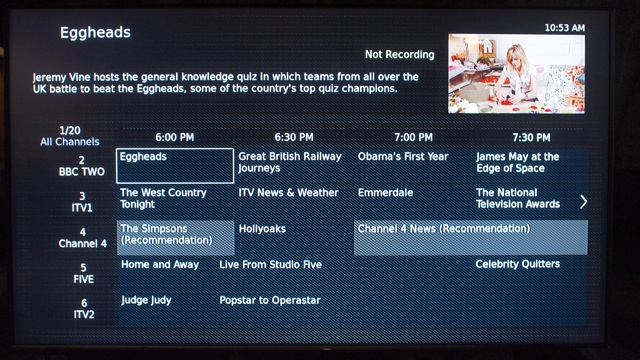
\includegraphics[width=6in]{mythtv-recommendations.jpg}
\caption{Recommendations appearing in MythTV frontend EPG} \label{fig:mythtv-recommendations}
\end{center}
\end{figure}

\begin{figure}[htbp]
\begin{center}
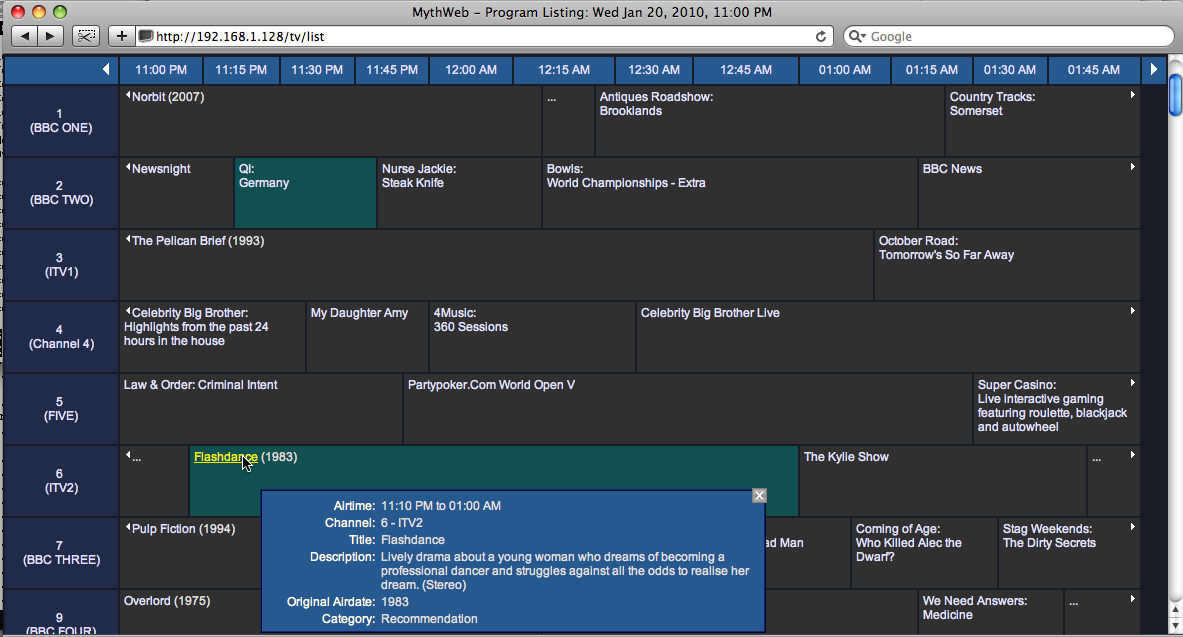
\includegraphics[width=6in]{mythweb-screen.png}
\caption{Recommendations appearing in MythTV web frontend (MythWeb)} \label{fig:mythweb-recommendations}
\end{center}
\end{figure}

\subsection{Scenario 2: Bookmark a Programme to the Web}

The screenshots in Figures \ref{fig:bot} and \ref{fig:bookmarks} show our proof of concept we used a text-based XMPP interface via MythTV to create bookmarks in delicious.com. XMPP is used where http would also work because we want to explore XMPPs built-in `friending' mechanism in later iterations for security and privacy. The user would not be expected to type the commands in manually in the finished interface.

\begin{figure}[htbp]
\begin{center}
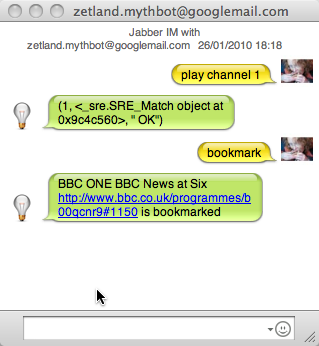
\includegraphics[width=3in]{bot.png}
\caption{Jabber bot communication with MythTV and Delicious} \label{fig:bot}
\end{center}
\end{figure}

\begin{figure}[htbp]
\begin{center}
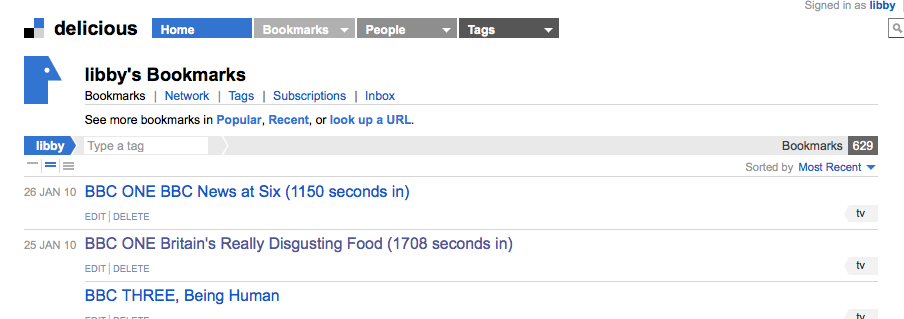
\includegraphics[width=6in]{bookmarks.png}
\caption{TV bookmarks appearing in Delicious} \label{fig:bookmarks}
\end{center}
\end{figure}

\subsection{Summary}

These experiments have satisfied us that the approach taken is workable, and we will continue to use the requirements, wireframes and scenarios to develop the prototype further.

\section{Evaluation}

From section 1, this workpackage's goal is to:

\begin{itemize}
\item{{\bf Enhance TV user experience by helping users find content they enjoy by making TV more social}}
\end{itemize}

by 

\begin{itemize}
\item{{\bf Being able to flexibly and quickly demonstrate ideas in a compelling fashion}}

\item{{\bf Allowing users to share information and recommendations and create textual user generated content - essentially metadata about television - using appropriate social media tools}}

\item{{\bf Enabling users to share their profile information while respecting user privacy}}

\item{{\bf Tested with BBC content}}
\end{itemize}

\subsection{Enhance TV User Experience}

We hope this document demonstrates that we have laid the foundations for achieving the goal of making TV more social, by connecting the TV with the Web and allowing data to flow in and out of the media centre environment through the `NoTube Network'. 
\\

\noindent{{\bf Helping users find content they enjoy and making TV more social}}
\\

This free flow of metadata means that online communities need not be segmented by region, and connections can be made with others beyond the geography of one's immediate TV network reach. In many cases we have used existing media centre functionality and extended it out further into the web, using HTTP APIs and protocols to liberate and reuse the user's data, while keeping it under their control. We have used `social' both in the local and networked senses, to help tie the usecases into compelling scenarios for very connected individuals but also taking into account that broadcast is by orders of magnitude the preferred medium for TV consuming.

In Scenario 2, wanting to know something more about a programme and remembering it for later is the key idea, a desire common to many TV watchers, regardless of the technologies they use. In Scenario 1, the filtering interesting programmes and bringing them to the user�s attention is the most important aspect, and one becoming increasingly relevant to all TV watchers as channels proliferate. 
\\

\noindent{{\bf Being able to flexibly and quickly demonstrate ideas in a compelling fashion}}
\\

We have used Open Source tools with existing user bases to enable rapid prototyping, and we plan to contribute useful code back to these projects where necessary. 
\\

\noindent{{\bf Allowing users to share information and recommendations and create textual user generated content - essentially metadata about television - using appropriate social media tools}}
\\

We have shown how users can create annotations and tags using appropriate input devices, which can then be used as input to social media tools. What is very significant here is that users can connect with their existing social networking sites to use the content they create socially.
\\

\noindent{{\bf Enabling users to share their profile information while respecting user privacy}}
\\

The Beancounter profile generator lays the foundations for profile sharing.
\\

\noindent{{\bf Tested with BBC content}}
\\

We have used the unique features of the BBC's web output, in particular URLs for programmes and publicly available structured metadata about programmes, to link the user's broadcast and on-demand TV watching with the web for BBC output.

\section{Next steps}

The next steps will be to {\bf improve the demonstrators} and {\bf fully document the APIs and formats used}, including working with APIs and other players, for example web-based HTML5 ones.

Slightly longer term there are significant pieces missing, in particular:
\\

\noindent{{\bf Privacy and Security}}
\\

We have a great deal of work to do in the area of securely logging into a TV system using a device and passing credentials from that device to other services. Similarly, being able to securely allow access to private data by other applications has not yet been implemented, although oAuth is a good candidate technology to use.

Having a permissions-based system for use of your TV with appropriate safeguards and non-intrusive user experience is another big piece to work on, although we have laid the groundwork by using a commonly-owned consumer device as a sophisticated remote control using the XMPP protocol.
\\

\noindent{{\bf Archival content}}
\\

We have concentrated largely on broadcast TV in the first iteration. In the next we will look at archival content and how recommendations can be used to surface this often hidden content.

\begin{figure}[htbp]
\begin{center}
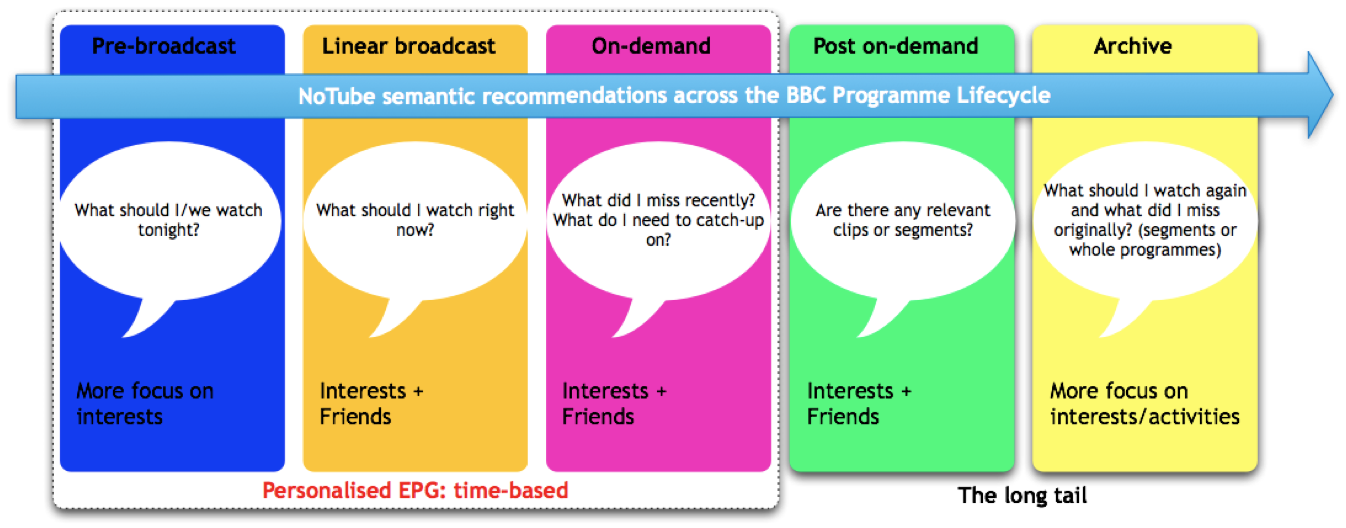
\includegraphics[width=6in]{archive-etc.png}
\caption{Recommendations through the lifecycle of content} \label{fig:archival}
\end{center}
\end{figure}



\appendix

\chapter{Appendix 1: Scripts}

These scripts are detailed walkthroughs of scenarios written as scripts where the components themselves as well as the users appear as characters with lines. This is an experiment to try to draw out the detail of the scenarios in order to create software and hardware components requirements and tasklists. The result is the swimlane diagrams included in the main text above.

\section{Scene 1: Watching recommendations for broadcast content: previous registration with the Beancounter Profiler}

\begin{verbatim}

INTERIOR. JANA'S SITTING ROOM - EVENING. TV IS OFF. JANA'S BOYFRIEND 
STEPHEN IS IN THE ROOM TYPING ON HIS LAPTOP.

JANA, age 34, enters the room, slumps on the sofa and looks at her phone. 

            JANA (grumbling) 
            There's nothing on. Again.

JANA switches on the MEDIA CENTRE anyway using the IPHONE

            IPHONE (to MEDIA CENTRE)
            Hi! I'm a known and trusted device belonging to JANA. Here are my 
            credentials. Please turn yourself on.
            
            MEDIA CENTRE (to IPHONE)
            Ok!

MEDIA CENTRE starts at the channel it was left in

            MEDIA CENTRE (to RECOMMENDER)
            Please tell me what JANA might like to watch now and later 
            this evening. 
            I'm a media centre, I'm being used by JANA, and the time is 19:30. 
            I'm in the UK. Here are JANA's credentials.
             
            RECOMMENDER (to PROFILE STORE)
            Please give me JANA's current profile. Here are JANA's credentials.
            
            PROFILE STORE (to RECOMMENDER)
            Ok! here you go. here's JANA's age, sex, gender, and some interests 
            (channels, brands and genres etc) that she likes. They were 
            calculated earlier today.
             
            RECOMMENDER (to PROFILE STORE)
            Thanks!

RECOMMENDER Calculates some things for JANA to watch this evening

            RECOMMENDER (to MEDIA CENTRE)
            Here's a channel to start with
            Here's some programmes for later 

MEDIA CENTRE shows some information about the recommended channel and 
programmes for later as the information becomes available as an overlay 
over what is currently playing. It also updates its EPG to show the 
recommendations for JANA as highlighted.

JANA flips to the suggested channel, then ignores the TV, opens her LAPTOP 
and starts sending a few emails. 

            IPHONE (to MEDIA CENTRE)
            Please change to the selected channel.

Around 20:00 JANA flips to the augmented EPG and sees Springwatch which is 
just starting.

            IPHONE (to MEDIA CENTRE)
            Please change to the EPG screen.
            
            MEDIA CENTRE (changing screen)
            Done. 

            JANA 
            STEPHEN, do you mind if I watch this thing with Bill Oddie?
            
            STEPHEN
            Nah, go for it. Wouldn't mind watching The Daily Show in half 
            an hour though.

JANA flips to Springwatch and watches TV.

            IPHONE (to MEDIA CENTRE)
            Please change to the selected channel.
            
            MEDIA CENTRE (to IPHONE, while changing channel)
            Done. I'm now watching Springwatch, PID b123456, channel is BBC1.

IPHONE looks up some interesting information about Springwatch and related 
items using THE BORE and makes them available for display if required.

            MEDIA CENTRE (to ACTIVITY STREAM GENERATOR)
            I'm now watching Springwatch, PID b123456, channel is BBC1, 
            user is JANA.

            ACTIVITY STREAM GENERATOR (to USER PREFERENCE CONTROLLER)
            What are JANA's user preferences?
            
            USER PREFERENCE CONTROLLER (to ACTIVITY STREAM GENERATOR)
            She puts all events including watch events in her public 
            activity stream

            ACTIVITY STREAM GENERATOR (to USER PREFERENCE CONTROLLER)
            Thanks. 

ACTIVITY STREAM GENERATOR adds Springwatch to JANA's public Activity Stream.
\end{verbatim}

\section{Scene 2: Bookmarking a TV show} 

\begin{verbatim}
INTERIOR. JANA'S SITTING ROOM - EVENING. TV IS ON AND JANA IS WATCHING 
SPRINGWATCH. JANA'S BOYFRIEND STEPHEN IS IN THE ROOM STILL TYPING 
ON HIS LAPTOP AND NOT REALLY WATCHING.

The time is around 20:23. JANA notices a type of bird she's particularly 
interested in on Springwatch.

            JANA (to no-one in particular)
            Ooh, I've been meaning to find out about Arctic terns because 
            of my trip to Shetland.

JANA quickly taps the 'TV bookmark' button on her IPHONE

            IPHONE (to MEDIA CENTRE)
            JANA bookmarked the thing playing now a few seconds ago.
            
            MEDIA CENTRE (to IPHONE)
            Ok I have bookmarked Springwatch, PID b123456, channel is BBC1, 
            23m33s in.

MEDIA CENTRE displays a discreet UI component stating that a bookmark 
has been created, which disappears after a few seconds.

            MEDIA CENTRE (to ACTIVITY STREAM GENERATOR)
            JANA bookmarked Springwatch, PID b123456, channel is BBC1, 23m33s in.
            
            ACTIVITY STREAM GENERATOR (to USER PREFERENCE CONTROLLER)
            What are JANA's user preferences?
            
            USER PREFERENCE CONTROLLER (to ACTIVITY STREAM GENERATOR)
            She puts all events including bookmark events in her 
            public activity stream

            ACTIVITY STREAM GENERATOR (to USER PREFERENCE CONTROLLER)
            Thanks. 

ACTIVITY STREAM GENERATOR adds Bookmarked Springwatch with the 
time to JANA's public Activity Stream.
\end{verbatim}

\section{Scene 3: Creating and playing playlists}

\begin{verbatim}
INTERIOR. DAYTIME. STEPHEN IS EATING LUNCH AT HIS DESK AND BROWSING THE WEB.

STEPHEN spots an interesting tweet:

"Clive Sinclair comes across as mister angry in #micromen, I met him 
once & he was lovely. Still have my speccy, but BBC Micro 
rox0rz too :-D" --rainycat 

STEPHEN searches for `micromen' and finds the BBC site. It's 
available on iplayer but he doesn't want to watch it right now. He 
adds it to his media centre playlist for later.

STEPHEN clicks on a bookmarklet in his browser

            BOOKMARKLET (to STEPHEN's MEDIA CENTRE)
            I'm acting on behalf of STEPHEN. Here are STEPHEN's credentials 
            and the URL of a programme. Please add the programme 
            to STEPHEN's playlist.
            
            MEDIA CENTRE (to BOOKMARKLET)
            Ok - done!
            
            MEDIA CENTRE (to THE BORE)
            Please find out some more about micromen for me.


            ~~~~~~~~~~~~~~~~


INTERIOR. JANA'S SITTING ROOM - EVENING. TV IS ON BUT NEITHER JANA 
NOR STEPHEN ARE REALLY WATCHING.

The time is 23:15. 

            STEPHEN (to JANA)
            Shall we watch something?
            
            JANA
            Yeah let me just finish this blog post. 2 minutes.

STEPHEN picks up his own IPHONE and starts browsing his playlist

            IPHONE (to MEDIA CENTRE)
            Hi! I'm a known and trusted device belonging to STEPHEN. 
            Here are my credentials. Please give me his playlist, 
            ordered by most recent.
                    
            MEDIA CENTRE (to IPHONE)
            Ok! Here you go.
            
            STEPHEN (to JANA)
            Ooh, fancy watching this Micromen thing?
            
            JANA (distractedly)
            Who's in it?
            
            STEPHEN
            Hang on

STEPHEN clicks on 'more info' button next to the Micromen playlist on his IPHONE.

            IPHONE (to THE BORE)
            Did you get those results back about micromen? can I have them?
            
            THE BORE
            hi! yep: it's got Alexander Armstrong out of Armstrong and 
            Miller in it. It's about computers in the UK in the 1980s. 
            The Guardian recommends it. There's 10 hours left to 
            watch on iPlayer.
            
            STEPHEN (to JANA)
            The guy out of Armstrong and Miller. Looks pretty good.
            
            JANA (saving the blog post)
            Ok! let's go for it.

STEPHEN clicks play on his IPHONE and they close laptops and 
watch the video on the MEDIA CENTRE. 

IPHONE (to MEDIA CENTRE)
Hi! I'm still a known and trusted device belonging to STEPHEN. 
Here are my credentials. Please play Micromen (b00n5b92) from 
STEPHEN's playlist.

MEDIA CENTRE (to IPHONE)
Ok! I'm now streaming Micromen.

            MEDIA CENTRE (to IPHONE, while changing channel)
            Done. I'm now playing Micromen, PID b00n5b92, channel is BBC4.

            MEDIA CENTRE (to ACTIVITY STREAM GENERATOR)
            I'm now watching Micromen, PID b00n5b92, channel is BBC1, 
            user is STEPHEN.

            ACTIVITY STREAM GENERATOR (to USER PREFERENCE CONTROLLER)
            What are STEPHEN's user preferences?
            
            USER PREFERENCE CONTROLLER (to ACTIVITY STREAM GENERATOR)
            He doesn't put watch events in his public activity stream.
            
            ACTIVITY STREAM GENERATOR (to USER PREFERENCE CONTROLLER)
            Thanks. 

ACTIVITY STREAM GENERATOR does nothing.
\end{verbatim}


\chapter{Appendix 2: Standards, APIs and Protocols}

\section{Buttons Protocol}

The Buttons protocoll\footnote{\url{http://wiki.foaf-project.org/w/Buttons}} is an independent project which uses the XMPP protocol to identify and control media services. It can be used by remote-control-like devices to discover and control services on the local network, in the local physical environment or on a remote network.

The rationale for using it is to provide a means for trusted devices to control local media devices, enabling remote devices to be written with greater functionality and flexibility. For example one could imagine a remote belonging to a friend hosted in a smartphone being used to control someone else's TV; or a smart phone app allowing browsing of EPG data as well as being able to change channel. Buttons is not restricted to television-related functionality but this is how we use it in this project.  


\section{EPG Filtering format and API}

This format is not currently sufficiently specified, although I give some indication below of what it might look like. The requirement is that the output of a recommendation engine can be applied to (a) an EPG and (b) a set of programmes available for download. The result is that the UI is able to filter the available programmes to show the user the programmes he or she will be interested in. the filter must also provide explanations for display to the user about `why this was recommended to you'.

The rationale is that recommendations need to work with a familiar interface and in the main interface - not tucked away in a hidden menu, but using the main UI of the media centre.

Example: Filter by a list of programme identifiers

\begin{verbatim}
http://example.com/recommendations/for/libby?date=2009-11-13

[
{
 "url":"http://www.bbc.co.uk/programmes/b00ny3mx",
 "title":"Andrew Marr's The Making of Modern Britain",
 "type":"broadcast",
 "channel":"http://www.bbc.co.uk/bbctwo/",
 "date":"2009-11-13 19:00:00",
 "reason","You have watched other programmes in this series."
 },
{
 "url":"http://www.bbc.co.uk/programmes/b00n5b92",
 "title":"Micro Men",
 "type":"on demand",
 "available_until","2009-12-13",
 "reason","Several of your friends have watched this programme 
   and you like programmes about computers"
 }
]
\end{verbatim}


\section{Identification of programmes and datamodel}


In general we follow the principles and detail of the BBC programmes Ontology.

\subsection{Distinguish Brand, Series, Programme, Version and Broadcast}

The Brand (e.g. `Doctor Who') and the Series (`Doctor Who season 8') must be distinguishable in some fashion from the specific programme (`Doctor Who season 8 programme 1'), and the specific version (`Doctor Who season 8 programme 1 signed version') that was broadcast on a specific date (a link between a version, a channel and a date-time). These different conceptual variants must be linked together.

The aims of this are: 

\begin{itemize}
\item{To be able to link similar but not identical versions of programmes (e.g. my annotation on an English subtitled version of the film 'Intacto' might still be interesting to a Spanish speaker).}
\item{To be able to make simple recommendations based on brands and series}
\end{itemize}

\subsection{Brand, Series, Programme, Version and Broadcast must have unique dereferenceable Web identifiers}

This is to link the programme with the Web. Where no web location is available we can for the moment drop the dereferencing requirement, but there still should be a unique URL for every programme.

The requirement for uniqueness is that the system must be able to identify whether a user has watched a specific programme or not. 

The requirement for de-referencability is that the system must be able to find out information about a programme even when the video content is not available.

\subsection{Channels must have unique dereferenceable Web identifiers}

One of the biggest benefits of NoTube could be a set of globally unique identifiers for channels, as that's the part where short names are often used and there is potential for confusion and failed lookups.

The aim here is to be able to do broadcast lookups in legacy systems.

\subsection{Good timekeeping}

By good timekeeping we mean care with timezone offsets; precision with date-times of broadcast, and agreement on date-time formatting.

The aim here is to be able to do broadcast lookups in legacy systems.

\subsection{Be able to identify points and time-based segments in video}

The aim here is to be able to annotate parts of Versions of Programmes with tags.

\subsection{Be extensible}

The aim is to be able to use other metadata formats where they have specific domain knowledge that we may not want to replicate, for example to be able to include a specific thesaurus for searching.


\section{Activity data}

The Atom activity model is based on the Atom Activities In RDF work and is as described in the deliverable D3.1. The draft RDF schema is available online: \url{http://xmlns.notu.be/aair#}

\section{User model description and APIs}

The user model and format is as described in the deliverable D3.1, and the RDf schema is available online: \url{http://xmlns.notu.be/wi#}

Here's a simplified, shortened user profile using a weighted interests\footnote{\url{http://xmlns.notu.be/wi}} approach, expressed in N3 RDF format as additions to FOAF\footnote{\url{http://xmlns.com/foaf/spec/}}, and assuming just one context (`working') for one person, Libby.

\begin{verbatim}
@prefix foaf: <http://xmlns.com/foaf/0.1/> .
@prefix wi: <http://xmlns.com/wi#> .
@prefix days: <http://ontologi.es/days#> .
@prefix tl: <http://perl.org/NET/c4dm/timeline.owl#> .
@prefix xsd: <http://www.w3.org/2001/XMLSchema#> .
@base <http://xmlns.com/wi#> .
    <http://swordfish.rdfweb.org/people/libby/rdfweb/webwho.xrdf#me>
    a foaf:Person;
    foaf:name "Libby Miller";
    foaf:gender "female";
    foaf:based_near [ geo:lat 48.402495; geo:long 2.692646 ];
    wi:preference [
      a wi:WeightedInterest;
      wi:topic <http://www.bbc.co.uk/5live#service>;
      wi:weight "3";
      wi:scale "0..9";
      wi:context <#working>
      ] ;
    wi:preference [
      a wi:WeightedInterest;
      wi:topic <http://www.bbc.co.uk/radio4#service>;
      wi:weight "7";
      wi:scale "0..9";
      wi:context <#working> .
      ] .
   <#working> a wi:Context;
       wi:timePeriod [
          a days:WeekdayInterval;
          tl:at "08:00:00"^^xsd:time ;
          tl:end "19:00:00"^^xsd:time .
       ] .

\end{verbatim}

\begin{verbatim}
I prefer radio 4 over radio 5 when I am working at home (which is every weekday 
between 8am and 7pm).
\end{verbatim} 

This expresses a simple ordering in the context of working for Libby in terms of channels, although a similar ordering could be expressed in terms of (for example) genres.


\end{document}
